\vspace{-1mm}
\section{Introduction}
\label{sec:introduction}
% what is the problem? Because of the large number of parameters, the generation of llm is slow and low utilizaiton. Serious problem in deployment.  
% Large language models (LLM), such as GPT3, PaLM show significant advantages for almost all aspects of natural language processing applications. The immense scale of the parameters unleashes the great potential of LLMs in various downstream tasks~\cite{bommasani2021opportunities,liang2022holistic}. The unprecedented model scale makes efficient LLM inference extremely challenging. Recently, several algorithms have been proposed from the established efficient inference directions, pruning, or quantization and achieved an impressive latency speed up of around $2 \times$. However, the reduction is not significant with respect to the rapid growth of model size.



% ideally, we have (i) does not require retraining (ii) LLM zero-shot in-context learning ability (iii) hardware efficient. 

% Our insgihts: if you can decide the sparsity pattern when doing the ocmputation for each weight. 

% Inspired by classic branch predictor, we envision a new way to sparsity on LLMs at inference-time:

% context-dependent sparsity: 

% challenge: 1. does it exist? 2. can we predict it fast and accurately? 3. can we exploit the prediction and use it reduce the latency in wall-clock time on hardware.  

% 1. how do we figure out if it exits. Discovery

% 2. observation residual: 

% 3. memory bound: io-aware sparsity. understand how hardware works, conceptually simple. flops/memory. 10->3x slower, will not have any speedup.
% io has to be blocked and contiguous. 

% hf
% metaseq
% that 

Large language models (LLMs), such as GPT-3, PaLM, and OPT have demonstrated that an immense number of parameters unleashes impressive performance and emergent in-context-learning abilities---they can perform a task by conditioning on input-output examples, without updating their parameters~\cite{bommasani2021opportunities,liang2022holistic,brown2020language,min2022rethinking,chan2022data}. However, they are very expensive at inference time, especially for latency-sensitive applications~\cite{pope2022efficiently}. An ideal inference-time model should use less computation and memory while maintaining the performance and special abilities of pre-trained LLMs. The simplest and most natural approach is sparsification or pruning, which has a long history before the LLM era~\cite{lecun1989optimal}. Unfortunately, speeding up inference-time sparse LLMs in wall-clock time while maintaining quality and in-context learning abilities remains a challenging problem.

% The recent advances in pre-trained large language models (LLM), such as GPT3, PaLM, and ChatGPT have suggested that the immense scale of parameters unleashes the great potential of language models -- they generalize well and achieve impressive performance on text generation and many downstream tasks~\cite{bommasani2021opportunities,liang2022holistic,gpt,opt,bloom,copilot,chatgpt}. However, they are very expensive at the inference-time deployment. An ideal inference-time model should use less compute and memory while retaining the generalization benefits of pre-trained LLMs. The most natural and simplest approach is sparsification or pruning, which has a long history before LLM era~\cite{lecun1989optimal}. Unfortunately, significantly speeding up inference-time sparse LLMs in wall-clock time without degrading the quality remains an unresolved problem.

% The unprecedented model scale makes efficient LLM inference extremely challenging. Recently, several algorithms have been proposed from the established efficient inference directions, pruning, or quantization and achieved an impressive latency speed up of around $2 \times$. However, the reduction is not significant with respect to the rapid growth of model size.


% Several algorithms have been proposed for efficient LLM inference with wall-clock latency reduction, which is an impressive progress given the difficulties to gain actual latency speed-up on modern hardware. ( The best-known speed-up is around $1.6\times$). Unfortunately, it is still not enough give the fast-growing size. 
% however, they fail to achieve significant wall-clock time speed-up without quality degradation in coping with the giant model size. The best-known speed-up is around $1.6x$, which is not significant enough in response to the growing model size. 

% Efficient inference has been a well-studied problem for convolution to bert, .., and there are three most established directions: pruning, quantization, and distillation. However, the scale is entirely upgraded. LLMs are generally with hundreds of billions of parameters, which makes a lot of techniques prohibitive expensive such as iterative pruning and distillation.  Recently, a line of work investigating, inference at this scale, 


While sparsity and pruning have been well-studied, they have not seen wide adoption on LLMs due to the poor quality and efficiency trade-offs on modern hardware such as GPUs. First, it is infeasible to retrain or iteratively prune models at the scale of hundreds of billions of parameters. Thus, methods in iterative pruning and lottery ticket hypothesis~\cite{lee2018snip,frankle2018lottery} can only be applied to smaller-scale models. Second, it is challenging to find sparsity that preserves the in-context learning ability of LLMs. Many works have shown the effectiveness of task-dependent pruning~\cite{michel2019sixteen,bansal2022rethinking}, but maintaining different models for each task conflicts with the task independence goal of LLMs. Lastly, it is hard to achieve wall-clock time speed-up with unstructured sparsity due to its well-known difficulty with modern hardware~\cite{hooker2021hardware}. For example, recent development in zero-shot pruning like SparseGPT~\cite{frantar2023massive} finds 60\% unstructured sparsity but does not yet lead to any wall-clock time speedup.

% generalize well
% cheap to do
% actual speed up

% many approaches~\cite{child2019generating,liu2022halos} have focused on a specific module, such as quadratic attention matrices at training time or large output space due to the large vocabulary size. However, they are not necessarily the bottlenecks in LLMs at inference time. understand the dynamics of LLMs at hundreds of billions scale and their interactions with downstream tasks
% Therefore, in this paper, we focus on answering the question that if there exists a \textit{inference-time sparsification} framework that (i) builds a deeper understanding of LLMs, (ii) maintains the quality of LLMs, and (iii) leads to significant speed-up in wall-clock time?
% Fortunately, we observe the following interesting phenomenon of LLMs.

% An ideal sparsity for LLMs should (i) not require model retraining, (ii) preserve quality and in-context learning ability, and(iii) lead to significant speed-up in wall-clock time on modern hardware. Inspired by mechanistic interpretation of LLMs that liken neural networks to computer circuits~\citep{olsson2022context,elhage2021mathematical} and classical branch predictor~\citep{smith1998study}, we hypothesize that for different tokens the model might effectively take different branches through the network [this might sound too handwavy?]. In other words, although densely trained, LLMs might have sparse paths that route different tokens to different subsets of the models without affecting the output. 
\begin{figure}[]
  \vspace{-2mm}
  \centering
   \subfigure[Contextual Sparsity]{
    % 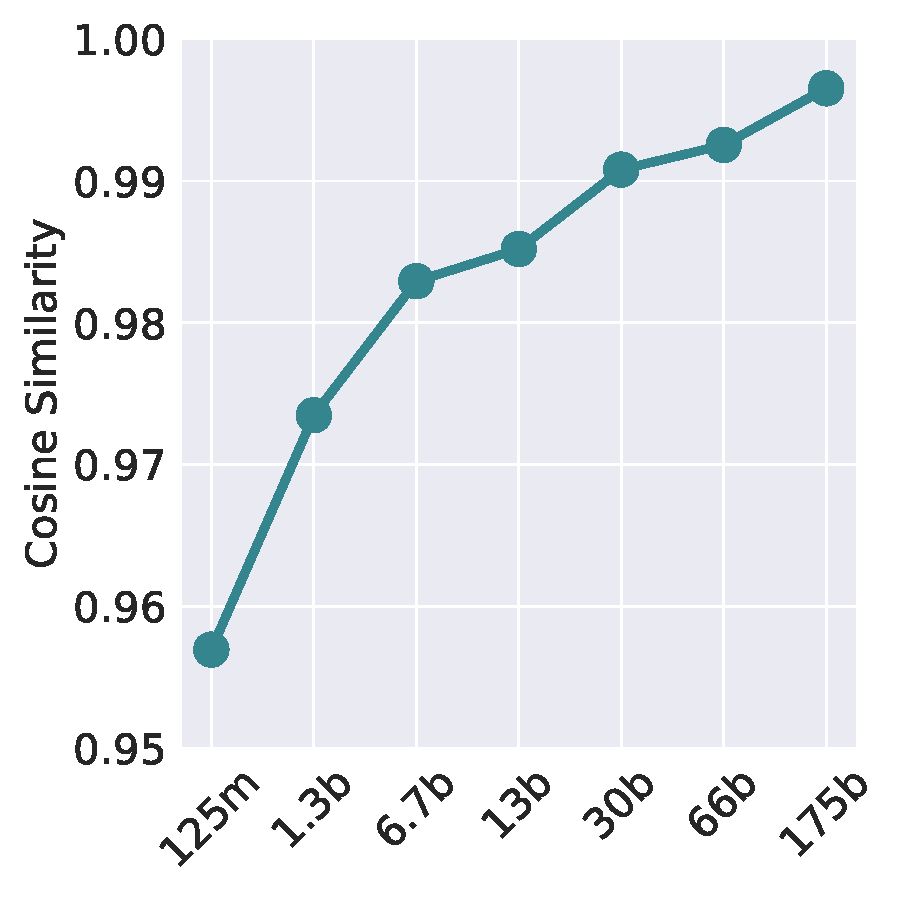
\includegraphics[width=0.22\textwidth]{figure/observation/cos_across_model.pdf}
    % \label{obs:slowlyevoloving-all}
    \hspace{0.5mm}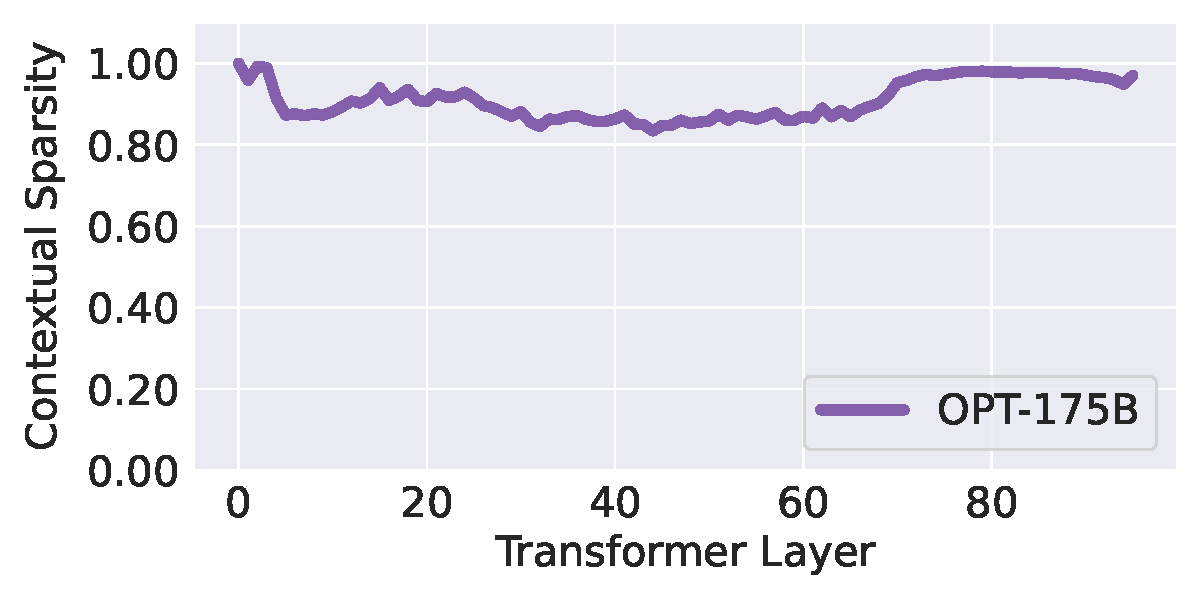
\includegraphics[width=0.398\textwidth]{figure/opt-175b-contextual-sparsity.pdf}
    \label{fig:sparsity-175}
    }\\
    \vspace{-3mm}
      % \hspace{0.5mm}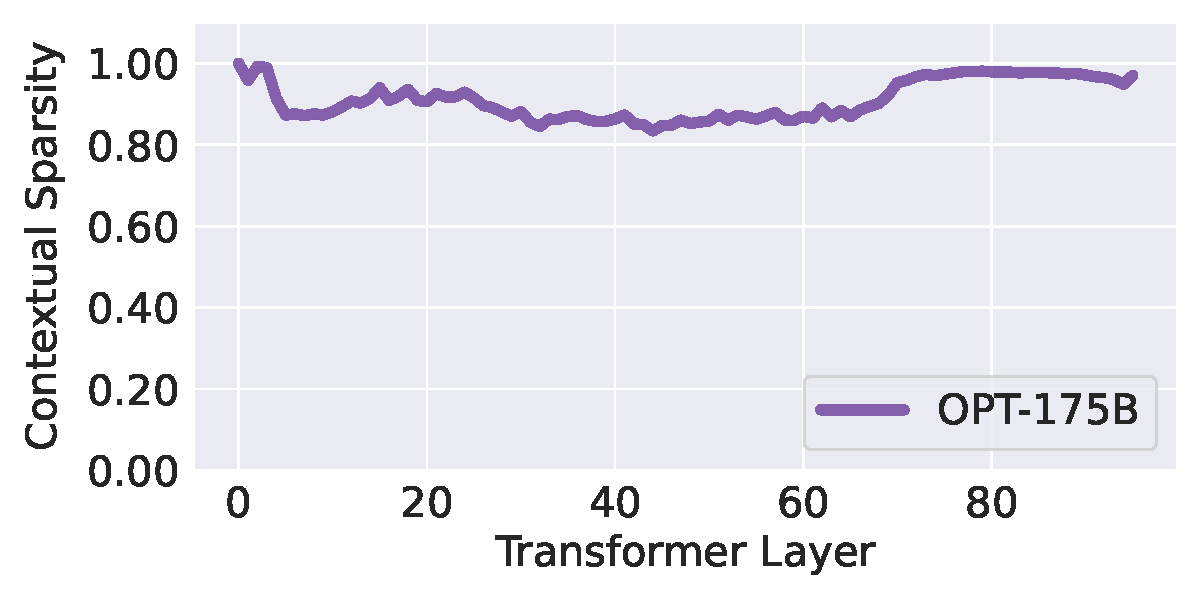
\includegraphics[width=0.398\textwidth]{figure/opt-175b-contextual-sparsity.pdf}
      \subfigure[Accuracy-Efficiency Trade-offs]{
    \hspace{-2mm}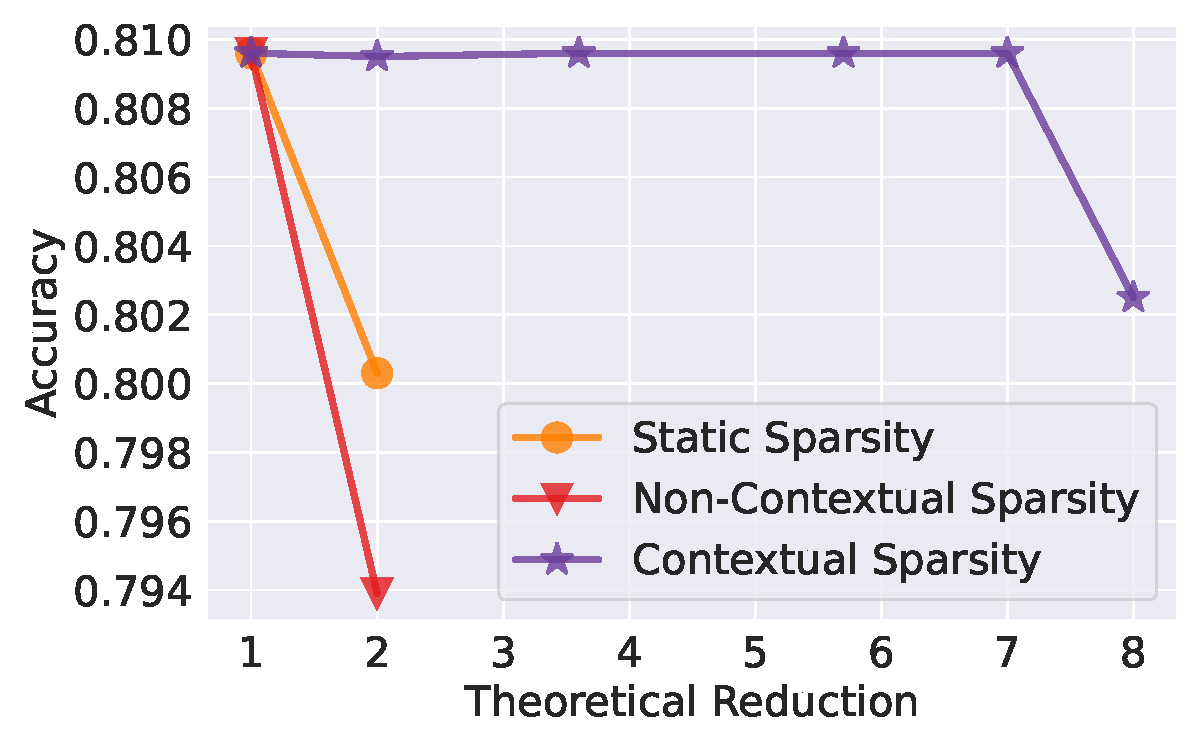
\includegraphics[width=0.4\textwidth]{figure/static-contextual-sparsity.pdf}
    \label{fig:sparsity-175-compare}
      }
      \vspace{-4mm}
  \caption{(1) LLMs have up to 85\% contextual sparsity for a given input. (2) Contextual sparsity has much better efficiency-accuracy trade-offs (up to 7$\times$) than non-contextual sparsity or static sparsity.}
    \vspace{-2mm}
  \label{fig:contextual-static} 
  \vspace{-2mm}
\end{figure}

An ideal sparsity for LLMs should (i) not require model retraining, (ii) preserve quality and in-context learning ability, and (iii) lead to speed-up in wall-clock time on modern hardware. To achieve such  demanding requirements, we go beyond \emph{static} sparsity in previous works (e.g., structured/unstructured weight pruning). We instead envision \emph{contextual sparsity}, which are small, input-dependent sets of attention heads and MLP parameters that lead to (approximately) the same output as the full model for an input. Inspired by the connections between LLMs, Hidden Markov Models~\citep{xie2022an, baum1966statistical}, and the classic Viterbi algorithm~\citep{viterbi1967error}, we hypothesize that for pre-trained LLMs,
\vspace{-2mm}
\begin{center}
\textit{\textbf{contextual sparsity} exists given any input.}
\end{center}
\vspace{-1mm}
The hypothesis, if true, would enable us to cut off specific attention heads and MLP parameters (structured sparsity) on the fly for inference-time, without modifying pre-trained models.
% Note that such a sparse path depends not only on individual input tokens (\emph{dynamic} sparsity) but also on their interactions (\emph{contextual} sparsity). The hypothesis, if it is true, will enable us to cut off specific neurons and/or heads on the fly for inference-time LLM inference, without modifying pre-trained models.
% while preserving the in-context learning ability, 
However, there are three challenges. 

    % \vspace{-0.2mm}
\underline{\emph{Existence}}: It is nontrivial to verify if such contextual sparsity exists, and naive verification can be prohibitively expensive. 
  \vspace{-0.1mm}
  
\underline{\emph{Prediction}}: Even if contextual sparsity exists, it is challenging to predict the sparsity for a given input in advance. 
  
  \vspace{-0.1mm}
\underline{\emph{Efficiency}}: Even if the sparsity can be predicted, it might be difficult to achieve end-to-end wall-clock time speedup. Taking OPT-175B as an example, the latency of one MLP block is only 0.2 ms on an 8$\times$A100 80GB machine. Without a fast prediction and optimized implementation, the overhead can easily increase the LLM latency rather than reduce it.

In this work, we address these challenges as follows:

\textbf{Existence}: Fortunately, we verify the existence of contextual sparsity with a surprisingly simple approach. To achieve essentially the same output, contextual sparsity is on average \textit{85\%} structured sparse and thereby potentially leads to a $7\times$ parameter reduction for each specific input while maintaining accuracy (Figure~\ref{fig:sparsity-175}). During explorations of contextual sparsity, we make important empirical observations and build a theoretical understanding of major components in LLMs that help address the prediction and efficiency challenge.

\textbf{Prediction}: We discover that contextual sparsity depends not only on individual input tokens (i.e., \emph{non-contextual} \emph{dynamic} sparsity) but also on their interactions (\emph{contextual dynamic} sparsity). Figure~\ref{fig:sparsity-175-compare} shows that with pure dynamic information, sparsity prediction is inaccurate. Only with token embeddings with sufficient contextual information can we predict sparsity accurately. Another finding is that \emph{contextual dynamic} sparsity for every layer can be predicted based on the ``similarity'' between layer parameters (heads/MLP) and the output from the previous layer, which carries the immediate contextual mixture of token embeddings.  

% The intuition is that, after training, the tokens that often co-occurr in the input sequences will tend to have similar embeddings. During inference, when the text input contains these co-occurred tokens, they will have high attention weights on each other. Therefore, after the first few layers of self-attentions, they will smooth their embeddings towards a common center. 


% we made a series of empirical observations and mathematical modeling to understand the major components of LLMs. 
%A contextual mixture of token embeddings are critical to making our prediction work

% such a prediction can be performed accurately, enabling our rolling prediction after a few initial layers.  

% here we need to connect with if we want to use contextual that was generated on the fly, we also need to make the prediction on the fly.  

\textbf{Efficiency}: Because at inference time, model parameters are static, inspired by the classical nearest neighbor search (NNS) literature and its applications in efficient deep learning, it is possible to formulate the above similarity-based prediction as an NNS problem~\cite{indyk1998approximate,zhang2018navigating,chen2020slide}. However, as mentioned, the overhead might be difficult to overcome as we would need to perform on-the-fly predictions before every layer. Luckily, we exploit a phenomenon of LLM where token embeddings change slowly across layers due to residual connections (well-known in computer vision~\cite{he2016deep}). Since the inputs to a few consecutive layers are very similar, we can design an asynchronous lookahead predictor (Figure ~\ref{fig:workflow_main}).



\begin{figure}[]
\vspace{-2mm}
  \centering
      \hspace{0.5mm}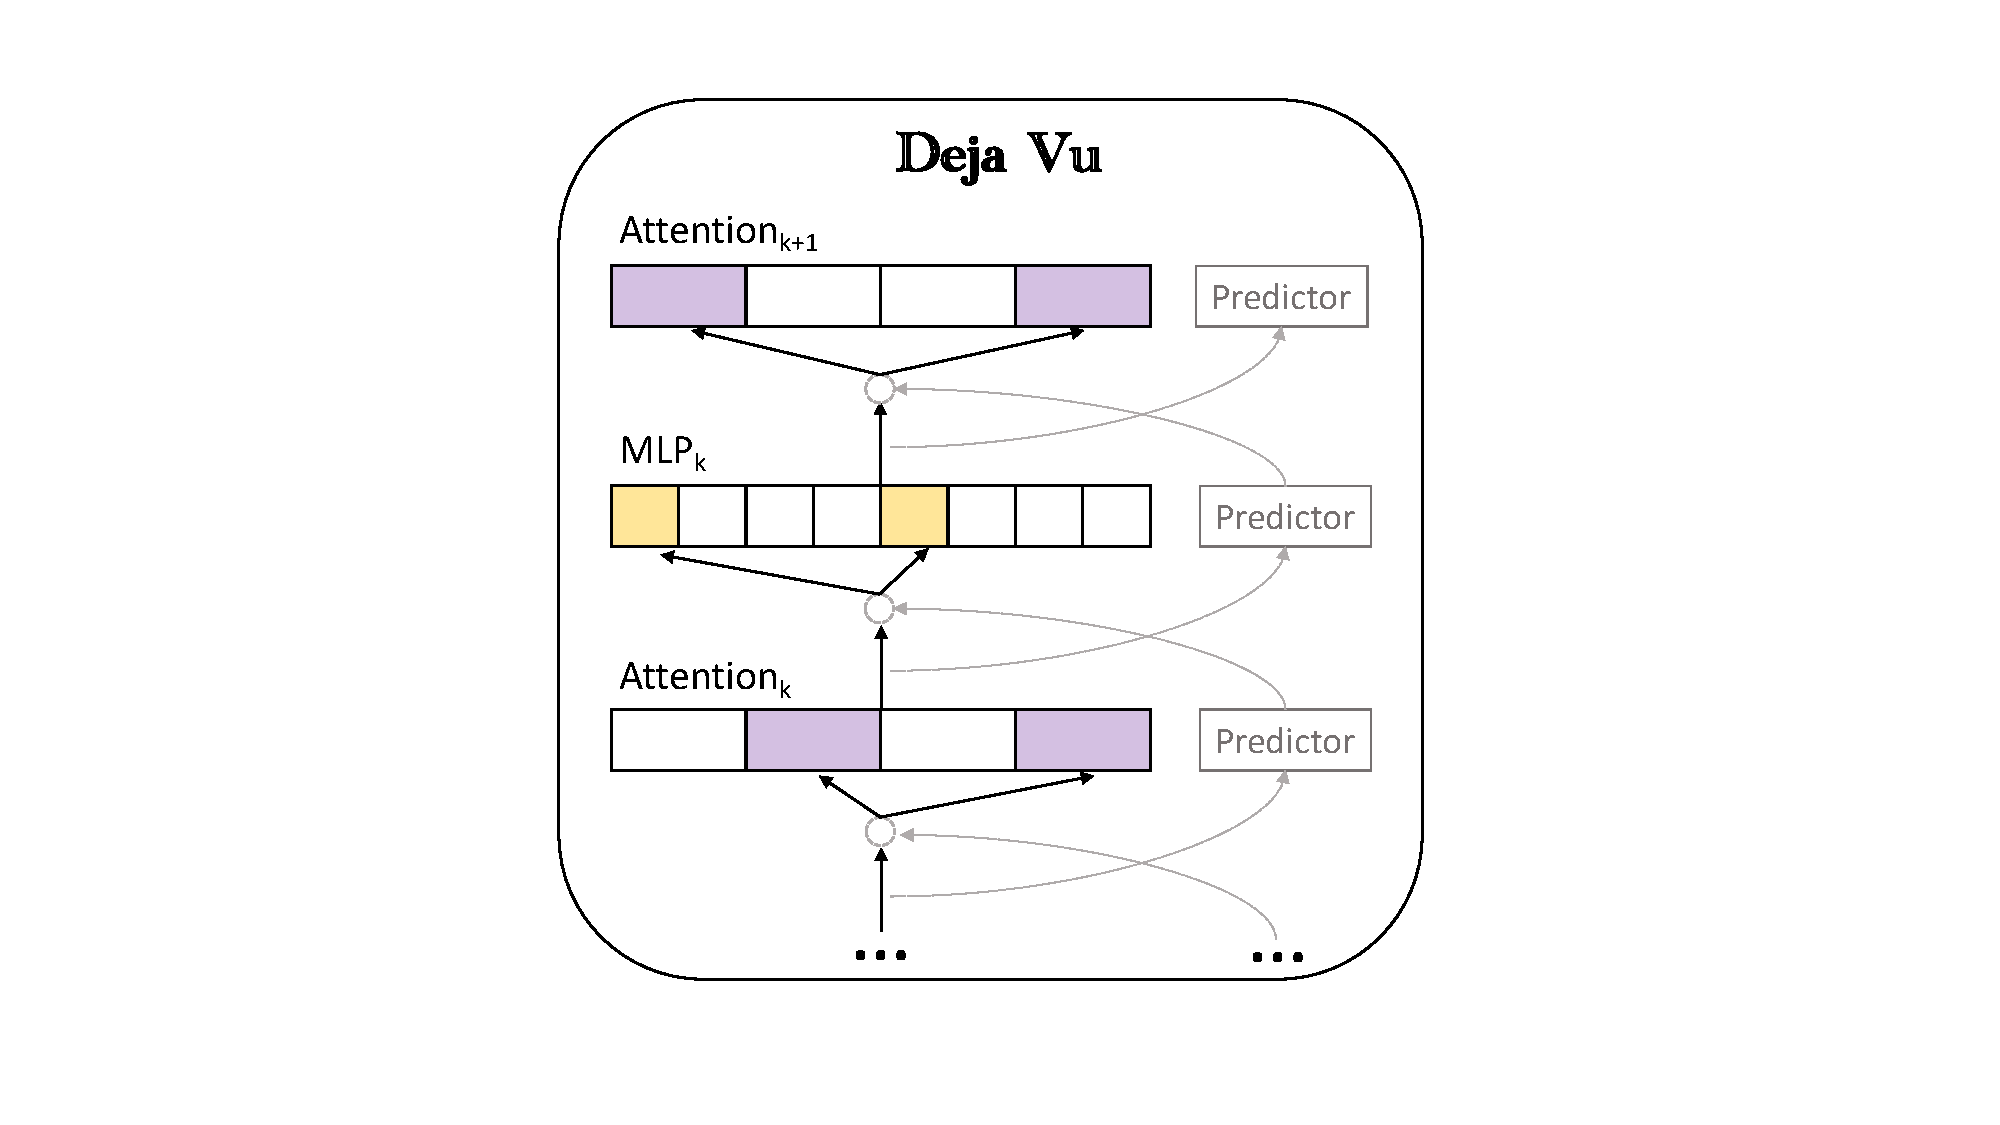
\includegraphics[width=0.34\textwidth]{figure/dejavu.pdf}
          \vspace{-3mm}
  \caption{\name{} uses lookahead predictors to side-step prediction costs: given the input to the attention layer at block $k$, they (asynchronously) predict the contextual sparsity for the MLP at block $k$, and given the input to the MLP at block $k$, they predict the sparsity for the attention head at the next layer.}
  \label{fig:workflow_main} 
    \vspace{-4mm}
\end{figure}

Based on our findings, we present a system, \name{}, that exploits contextual sparsity and realizes efficient LLMs for latency-sensitive applications.
\vspace{-0.7mm}
\begin{itemize}[itemsep=0.1pt,topsep=0pt,leftmargin=*]
\item  In Section~\ref{sec:routing_mlp} and Section~\ref{sec:routing_attn}, we present a low-cost learning-based algorithm to predict sparsity on the fly. Given the input to a specific layer, it predicts a relevant subset of attention (heads) or MLP parameters in the next layer and only loads them for the computation.
\vspace{-0.2mm}
\item  In Section~\ref{sec:hide_overhead}, we propose an asynchronous predictor (similar to classic branch predictor~\cite{smith1998study}) to avoid the sequential overhead. A theoretical guarantee justifies that the cross-layer design suffices for accurate sparsity prediction.
% \item After integrating low-level implementation such as fast SpMV in the PyTorch model.
    % \item  In section~\ref{sec:routing_mlp} and section~\ref{sec:routing_attn}, we propose a low-cost learning-based algorithm that can adaptively sparsify both attention and MLP blocks. Specifically, based on input to each layer,  our algorithm performs an on-the-fly prediction on a subset of attention (heads) and MLP parameters. Then only the predicted parameters are loaded for computation.
    
    % \item  In section~\ref{sec:hide_overhead}, we propose an optimized design (similar to classic branch predictor~\cite{smith1998study}) to avoid sequential overhead from sparsity predictor. We first observe that activation is slowly changing across layers (due to residual connection). We can exploit the similarities of activation in consecutive layers to asynchronously perform the sparsity prediction and hide its overhead. Finally, we provide a theoretical guarantee that the cross-layer design is sufficient for accurate sparsity prediction. 
    % \item In Section~\ref{sec:sparse_matmul}, we present a system that realizes the wall-clock time speed-up of LLMs. We integrate our low-level implementation such as fast SpMV in the PyTorch model and realize xx $\times$ speed up compared to C++ implemented fast transformer, which is the fastest inference-time LLM implementation so far.
\end{itemize}

% Furthermore, we are able to predict sparsity on the fly with low latency. First, we propose a low-cost learning-based algorithm (section~\ref{sec:routing_mlp} and section~\ref{sec:routing_attn}). Given the token embeddings computed after initial few layers, it predicts a relevant subset of attention (heads) and MLP parameters in the next layer on the fly, and only loads them to compute further embeddings. Second, due to residue connection, token embeddings change slowly across consecutive layers and thus such a prediction can extend to \emph{next few} layers (section~\ref{sec:hide_overhead}). As a result, this leads to a low-latency asynchronously rolling prediction. A theoretical guarantee justifies that the cross-layer design suffices for accurate sparsity prediction. 

After integrating hardware-aware implementation of sparse matrix multiply (Section~\ref{sec:sparse_matmul}), \name{} (written mostly in Python) can reduce latency of open-source LLMs such as OPT-175B by over 2$\times$ end-to-end without quality degradation compared to the state-of-the-art library FasterTransformer from Nvidia (written entirely in C++/CUDA), and over 2$\times$ compared to the widely used Hugging Face implementation at small batch sizes. Furthermore, we show several ablations on different components of \name{} and its compatibility with quantization techniques.

% a 7$\times$ speed up on MLP and a 3 $\times$ speed up on attention blocks. We demonstrate that our cross-layer sparsity prediction saves the sequential overhead by XX. At last, we verify that Deja Vu is compatible with quantization techniques without accuracy drops. 


% : on OPT-175B running on 8 A100 80GB machines, it is faster than loading one MLP block (0.2 ms).


% Note that a contextual mixture of token embeddings are critical to make our prediction work. We show that with pure dynamic information (e.g., individual input token embedding), the prediction is almost random and unusable; only with token embeddings that contain sufficient contextual information, such a prediction can be performed accurately, enabling our rolling prediction after a few initial layers.  

% After integrating low-level implementation such as fast SpMV in the PyTorch model (section~\ref{sec:sparse_matmul}), we present a system \textbf{Deja Vu} that realizes the wall-clock time speed-up of LLMs. When applied to open-source LLMs such as OPT-175B, we achieve up to 2 $ \times$ latency reduction end-to-end  without quality degradation compared to C++ implemented fast-transformer, which is the fastest inference-time LLM implementation so far, and 10 $\times$ latency reduction compared to Hugging Face (Section~\ref{sec:experitns}). Furthermore, we show several ablations on

% a 7$\times$ speed up on MLP and a 3 $\times$ speed up on attention blocks. We demonstrate that our cross-layer sparsity prediction saves the sequential overhead by XX. At last, we verify that Deja Vu is compatible with quantization techniques without accuracy drops. 

% Such compatibility implies the possibility of integrating two complementary directions to achieve both memory-efficient and fast LLMs at inference time.

\iffalse
In section, we propose an optimized design (similar to classic branch predictor~\cite{smith1998study}) to avoid sequential overhead from the sparsity predictor. We first observe . We can exploit the similarities of activation in consecutive layers to asynchronously perform the sparsity prediction and hide its overhead. 
\fi

% Leveraging such sparsity would need to be achieved in a shorter time span.  

%At last, even if the sparsity can be predicted, it is extremely hard to achieve end-to-end wall-clock time speedup. . Without a fast prediction and optimized implementation, the overhead can easily increase the LLM latency rather than reduce it.

% ideally, we have (i) does not require retraining (ii) LLM zero-shot in-context learning ability (iii) hardware efficient. 

% Our insgihts: if you can decide the sparsity pattern when doing the ocmputation for each weight. 

% Inspired by classic branch predictor, we envision a new way to sparsity on LLMs at inference-time:

% context-dependent sparsity: 

% challenge: 1. does it exist? 2. can we predict it fast and accurately? 3. can we exploit the prediction and use it reduce the latency in wall-clock time on hardware.  

% 1. how do we figure out if it exits. Discovery

% 2. observation residual: 

% 3. memory bound: io-aware sparsity. understand how hardware works, conceptually simple. flops/memory. 10->3x slower, will not have any speedup.
% io has to be blocked and contiguous. 

% hf
% metaseq

\iffalse
However, there are three challenges. First, it is unknown and expensive to verify if such an in-context sparsity exists, and naive verification can be prohibitively expensive. Second, even if it exists, it is challenging to predict the sparsity for a given input in advance.  At last, even if the sparsity can be predicted, it is extremely hard to achieve end-to-end wall-clock time speedup. Taking OPT-175B as an example, the latency of one MLP block is only 0.2 ms on 8 A100 80GB machines. Without a fast prediction and optimized implementation, the overhead can easily increase the LLM latency rather than reduce it.
\fi

% First, it is unknown how to or if it is possible to predict the sparsity for a given input in advance. In the above observation, we can identify the sparsity pattern only after performing a full LLM evaluation on each input. Second, due to the size of pre-trained LLMs, the prediction algorithm needs to have a light or scalable pre-processing step. Last, most importantly, even if there exists a prediction algorithm with cheap pre-processing time, it is very challenging to predict efficiently. Taking OPT-175B as an example, the latency of one MLP block is only 0.2 ms on 8 A100 80GB machines. The headroom is so tight that the overhead of the prediction algorithm can easily increase the LLM latency rather than reduce it.



% The above observation provides a huge opportunity to generate tokens $15\times$ faster.
% shows that on average each token only activates 5\% rows (or columns) in FFN matrices and 10\% of attention heads. Furthermore, since token generation latency is one of the major challenges of LLM deployment for its token-by-token serial computation (details in Section~\ref{sec:related_work}), the above observation provides a huge opportunity to generate tokens $15\times$ faster.

% challenges:  Especially it is unknown if the prediction is possible on attention modules, the most important building block of LLMs.
% However, there are three challenges to exploiting the above observation and speeding up LLMs at inference time. First, it is unknown how to or if it is possible to predict the sparsity for a given input in advance. In the above observation, we can identify the sparsity pattern only after performing a full LLM evaluation on each input. Second, due to the size of pre-trained LLMs, the prediction algorithm needs to have a light or scalable pre-processing step. Last, most importantly, even if there exists a prediction algorithm with cheap pre-processing time, it is very challenging to predict efficiently. Taking OPT-175B as an example, the latency of one MLP block is only 0.2 ms on 8 A100 80GB machines. The headroom is so tight that the overhead of the prediction algorithm can easily increase the LLM latency rather than reduce it.

% prediction overhead is extremely tight. 
% , which requires careful design and implementation to realize the theoretical gain. 

% (ii) How to predict: We can only identify the sparsity pattern after the full computation, which has no savings. Thus it is unknown if there exists an algorithm to accurately predict the sparsity pattern. (iii) How to speed up: even if we could predict the sparsity pattern only depending on the current input accurately, the overhead of the prediction might even increase the latency of token generation rather than speed it up. Taking OPT-175B as an example, the latency of MLP block is around 0.5ms on 6 A100 80GB machines. \emma{please check if 0.5ms is abound right}. The overhead budget is extremely tight, which requires careful design and implementation to realize the theoretical gain. 
% Moreover, although what we observe is structured sparsity (rows/columns and heads), it requires careful design and implementation to realize the theoretical gain.      Compared to $2\times$ parameter reduction by unstructured pruning~\cite{frantar2023massive}, 

\iffalse
To address the above challenges, we start with a series of empirical explorations and mathematical modeling to understand the major components of LLMs. The most important result is that we verify the existence of the above context-dependent sparsity with a surprisingly simple approach -- for a given input, its contextual sparsity is a set of attention heads and MLP parameters that produce high activation (Figure~\ref{}). This path is in average \textit{85\%} structured sparse and thereby provides a huge opportunity for a $7\times$ parameter reduction for each specific input while maintaining accuracy. 
% Thus, we verify the existence of in-context sparsity with two forward passes: In the first pass, we record the parameters that yield large residual norms; In the second pass, we pass the token only through these parameters. Surprisingly, these two forward passes lead to a similar prediction on various in-context learning tasks. We also verified that for different tokens, the passes they take through the model are different.
\fi

% We find that embedding evolves extremely slowly for models with hundreds of billions of parameters (due to residual connection~\cite{}).  As a result, one efficient signal for deciding in-context sparsity patterns is its impact on the residual norm. Thus, we verify the existence of in-context sparsity with two forward passes: In the first pass, we record the parameters that yield large residual norms; In the second pass, we pass the token only through these parameters. Surprisingly, these two forward passes lead to a similar prediction on various in-context learning tasks. We also verified that for different tokens, the passes they take through the model are different.


% We present several important findings along with theoretical models to understand major components of LLMs, such as MLP, attention, and residual connections. Then we show how they can unlock the possibility of performing an efficient sparsity pattern prediction. The following is an example of residual connections.

% \textbf{LLMs are context-dependent sparse}: Although densely trained, LLMs naturally have up to \textit{90\%} structured sparsity for every input depending on its context (Figure~\ref{observation:sparsity}). Specifically, compared to $2\times$ parameter reduction by unstructured pruning~\cite{frantar2023massive}, this observation provides a huge opportunity for a $10\times$ adaptive parameter reduction (structured) for each specific input while maintaining accuracy. 

% \textbf{Self-attention are clustering algorithms}: 

% During training, the input tokens that often co-occur in the input sequences will tend to have similar embeddings. During inference, when the text input contains these co-occurred tokens, they will have high attention weights on each other. Therefore, after the first few layers of self-attentions, they will smooth their embeddings towards a common center. 

% With this clustering idea in mind, when we want to predict which heads to use for the token $y_{t+1}$, given the embedding $x_{k,t}$ at layer k, by guessing (1) which heads are related to the embedding $x_{k,t}$ (this head will also be related to all other tokens in the same cluster), and (2) whether the next token to be predicted is related to those heads, we could predict what are the subset of heads to be used to predict the next token $y_{t+1}$. This is due to the residual architecture design for training stability~\cite{}.

% \textbf{Embeddings are slowly evolving } (Figure~\ref{observation:residual}): we observe that embeddings are slowly evolving along each layer at inference-time because residuals are small in pre-trained LLMs. Since embeddings in consecutive layers are very similar, we could asynchronously perform the sparsity prediction and hide its overhead, e.g., use embeddings for $10^{th}$ layer to predict the sparsity for $11^{th}$ layer, which provides the opportunity to address the aforementioned third challenge.

% In this paper, we first show detailed observations on \textit{inference-time structured sparsity} and provide a general formulation of the problem as \textit{inference-time structured sparsity search} in section. Then we present two empirical findings on multi-head attention and residual connection along with theoretical analysis, which shows the possibility of addressing all three challenges above. Specifically:
% \begin{itemize}[leftmargin=*,nosep,nolistsep,noitemsep]
% \item In section~\ref{sec:obs_att_cluster}, we find that \textit{inference-time structured sparsity} of current token generation does not hurt the quality of future generated tokens. To better understand this phenomenon, we visualize the attention heads and find that each head is likely to only cluster a few tokens together and others are scattered. Based on these, we present a unified theoretical understanding by viewing multi-head attention blocks as clustering algorithms. Intuitively, during training, the tokens that often co-occur in the input sequences will tend to have similar embeddings; as a result, these co-occurred tokens have high attention weights on each other at inference time.
% \item In section~\ref{sec:obs_slowly_changing}, we observe that both residual connections, one around the attention block and one around the MLP block, have very small norms, resulting in slowly evolving embedding along layers in LLMs. Then we present a theoretical analysis that explains when and why the residual norm shrinks along with a lower and upper bound. Intuitively, on the one hand, residuals are large enough to provide information signals; on the other hand, residuals are small enough to ensure slowly changing activation. 
% \item We can exploit the above in two ways: (1) we could learn a predictor for \textit{inference-time structured sparsity} and the training signal is the sparsity pattern that could maintain the norm of residuals (2) The upper bound of the \textit{small residual} inspires a system design that we could predict \textit{inference-time structured sparsity} with embeddings from a few layers before. Because of the high similarity between embeddings in neighbor layers throughout the model (Figure~\ref{observation:residual}). In this way we could ``hide" or overlap the prediction overhead.



% In section~\ref{}, we first observe that both residual connections, one around the attention block and one around the MLP block, are very small. we find that $\|F(X)\|$ is significantly smaller than $\|X\|$ and the cosine similarity between $X$ and $X'$ is extremely high . This results in slowly evolving embedding. because small values will be dominated by the skip connection


% \end{itemize}

\iffalse
Based on the above and other findings in Section~\ref{sec:obs}, we design Deja Vu - a inference-time context-dependent sparsity for reducing the latency of LLMs.
\vspace{-2.5mm}
\begin{itemize}
    \item  In Section~\ref{sec:routing_mlp} and Section~\ref{sec:routing_attn}, we propose a low-cost learning-based algorithm that can adaptively sparsify both attention and MLP blocks. Specifically, based on input to each layer,  our algorithm performs an on-the-fly prediction on a subset of attention (heads) and MLP parameters. Then only the predicted parameters are loaded for computation.

    
    % predicts the structured sparsity pattern at each MLP block using the input to the current transformer layer.  sparsifies a MLP layer; For Attention block, it adaptively select a few heads. the input to a subset of heads in the attention blocks and a subset of neurons in the FFN blocks at inference time. Specifically, the amount of contribution to the residuals is a natural signal for the importance of an attention head or neurons. Therefore, we collect these signals on a small amount of training data and learn a routing classifier for every block. The predictor operates only based on the current token without knowing the previous sequences thanks to the clustering behavior in the attention block.

    \item  In Section~\ref{sec:hide_overhead}, we propose an optimized design (similar to classic branch predictor~\cite{smith1998study}) to avoid sequential overhead from sparsity predictor. We first observe that activation is slowly changing across layers (due to residual connection). We can exploit the similarities of activation in consecutive layers to asynchronously perform the sparsity prediction and hide its overhead. Finally, we provide a theoretical guarantee that the cross-layer design is sufficient for accurate sparsity prediction. 
    
    % predict the sparsity pattern for the next layer using the embedding at the current layer, e.g., use embeddings for $10^{th}$ layer to predict the sparsity for $11^{th}$ layer. In this way, we could asynchronously perform the sparsity prediction and hide its overhead. We provide a theoretical guarantee that the cross-layer design is sufficient for accurate sparsity prediction. 

    % Since embeddings in consecutive layers are very similar, we could asynchronously perform the sparsity prediction and hide its overhead, e.g., use embeddings for $10^{th}$ layer to predict the sparsity for $11^{th}$ layer.
    % the embedding from the previous layers as the input to the sparsity predictor, exploiting the observation of slowly evolving embeddings. In this way, we can parallel routing prediction and layer computation. 
    % We provide a guarantee that with high probability, the predicted \textit{inference-time structured sparsity} by the earlier embedding proxy is very close to that by the actual input embedding.
    
    % \item In section~\ref{sec:sparse_matmul}, we present a system design that realizes the wall-clock time speedup of token generation of LLMs. 
    % First, we present a finding that although trained sequentially, attention and FFN blocks can also be paralleled at inference time.
    % It provides another degree of parallelism and reduces communication overhead. Then we demonstrate an optimized low-level implementation such as fast SpMV. 
    \item In Section~\ref{sec:sparse_matmul}, we present a system that realizes the wall-clock time speed-up of LLMs. We integrate our low-level implementation such as fast SpMV in the PyTorch model and realize xx $\times$ speed up compared to C++ implemented fast transformer, which is the fastest inference-time LLM implementation so far.
\end{itemize}
\fi

% In section~\ref{sec:experitns}, we demonstrate the utility and efficiency of Deja Vu on LLMs. When applied to OPT-175b, we show a 7$\times$ speed up on the MLP block and a 3 $\times$ speed up on the Attention block. We achieved the best-known end-to-end 3 $\times$ latency reduction on 8xA100 without quality degradation.  [reach goal] When combined with weight quantization techniques, we further reduce the latency by xxx.  

% One of the main reasons is that these proposals straightly apply ideas from long-standing efficient directions, either pruning or quantization. \cite{bansal2022rethinking, li2022large} observes high sparsity in LLMs and naturally approaches sparsity with the pruning technique. \cite{xiao2022smoothquant,dettmers2022llm} are motivated by the giant model size and applied quantization with a few technical improvements. Designing an inference framework for LLMs without diving into the model behavior is like walking in a maze based only past experience with eyes blindfolded. An ideal efficient LLM inference framework should be designed based on the understanding of model behaviors.

% This paper presents a series of observations and understandings of model behaviors at hundreds of billions of parameters. First, we observe not only high sparsity but also dynamic sparsity at the Softmax function in the Attention block and the activation function in the MLP block (Figure~\ref{observation:residual}). Second, for the two residual connections $X' = X + F(X)$ inside each transformer layer, one around the attention block and one around the MLP block,  we find that $\|F(X)\|$ is significantly smaller than $\|X\|$ and the cosine similarity between $X$ and $X'$ is extremely high (Figure~\ref{observation:residual}). This results in slowly evolving embedding. Third, we observe clustering behavior happening at the multi-head attention(Figure~\ref{observation:residual}). During training, the tokens that often co-occur in the input sequences will tend to have similar embeddings; as a result, these co-occurred tokens have high attention weights on each other during inference.




% Based on all these observations, we imagine inference-time architecture, with a routing algorithm that adaptively activates a few attention heads and a subset of MLP neurons that is important to a given test sample.  The magnitude of residuals $\|F(X)\|$ is a natural signal for the importance of an attention head or neurons. Small values will be dominated by the skip connection. Further, we can collect these signal and train a routing classifier for every block. The predictor operates only based on the current token without knowing the previous sequences thanks to the clustering behavior in the Attention block.  At last, the routing prediction can be made based on the embedding from the previous transformer layer because of the extremely slowing evolving activations. Sequential overhead is avoided when parallel routing prediction and layer computation.


% When it comes to efficient inference, there are three most established directions: pruning, quantization, and distillation. Unfortunately, it is challenging to achieve significant wall-clock time speed-up without quality degradation in coping with the giant model size. Specifically, pruning exploits model sparsity; however, speed up is difficult due to the complication on modern hardware from unstructured sparsity~\cite{frantar2023massive}, or requires prohibitive retraining cost~\cite{hanpruning}. Quantization focuses on memory reduction and does not lead to significant speed up in practice~\cite{xiao2022smoothquant,dettmers2022llm,frantar2022gptq}. Distillation is expensive at billion scale parameters without quality guarantee as it contradicts the observation on LLM's Moore's Law. 


% Recent studies on LLMs(~\cite{bansal2022rethinking, li2022large} all observe high sparsity in LLMs, both in attention Block and MLP blocks. Despite the extremely large number of parameters, it appears that only a part of the model is activated for a given input. Thus, we imagine an oracle for inference-time model routing, a method that adaptively chooses a part of models that is important to a test sample. Specifically, in LLMs, every transformer layer starts with an Attention Block and follows by an MLP Block. We envision a routing algorithm would compute only a few attention heads and a few MLP neurons but yield the same model output.

% LLMs are auto-regressive in nature, meaning that the activation depends on all previous sequences for a given token. Here, we ask the question, can the routing algorithm directly operate on the current token without knowing the previous history.?  For the MLP block, the answer is straightforward because the MLP block is not auto-regressive. For the Attention block, interestingly, the answer is still positive based on an understanding of the token mixture happening in the Attention Block. The intuition is that, after training, the tokens that often co-occur in the input sequences will tend to have similar embeddings. With this clustering characteristic, the routing algorithm would naturally activate similar heads; at the same time, these co-occurred tokens have high attention weights on each other during inference.

% As we remove the dependency on the previous context, we argue the possibility of such a routing algorithm. Practically, inference time routing opens opportunities for LLM efficient inference because it essentially reduces the model width for a test sample. Taking only the embedding of the current token as input, a routing predictor can be learned for each block to predict which head or neurons would yield a high activation magnitude.  Activation magnitude is a natural signal indicating the model components' importance. For an MLP layer, after the activation function, small values will be zeroed out. For a Multi-Head Attention layer, the output would be dominated by high attention weights head due to the softmax function.   However, there exist practical challenges. Such routing predictors introduce overhead because computation is paused when waiting for the routing decision.

% Luckily, inference time routing would still speed up inference latency based on our observation that embedding of a token evolves \emph{extremely slowly} in LLMs.
% We record the activation after the Attention block and the activation after the MLP block for all transformer layers.  We compute the cosine distance between these activations and find that, taking OPT-175b as an example, (1) the cosine similarity between the input of the Attention block and the MLP block within the same transformer layer is over 99\%. (2) the cosine similarity between the input of any two consecutive transformer layers is over 98\%. We show that the routing can be decided using activation from the previous layer such that  routing prediction and model computation can be paralleled to avoid sequential overhead. 

% We demonstrate that these slowly changing activations provide two opportunities to realize the
% ideal efficient inference framework. [missed why slowly changing allows the following solutions] First, to reduce the depth, we could introduce parallel computing into LLM's execution, for example, parallel the computation of the Attention block and MLP block. Second, to reduce the width, an algorithm can adaptively select a small set of neurons for computation to reduce the memory access and computation of MLP block given the high sparsity of MLP block, which we will discuss in detail in Section~\ref{sec}. However, this comes with
% two main challenges: (i) how to design a parallel strategy that avoids fine-tuning LLMs without losing accuracy, (ii) how to reduce the overhead introduced when dynamically selecting neurons.








% Assume the routing algorithm for one input sequence is obtained by recording which attention heads and MLP neurons yield high magnitudes; we find that for this sequence, such routing algorithm doesn't incur model quality degradation. 



% We first argue the existence of such a routing algorithm by understanding the token mixing nature in these auto-regressive models. Specifically, we ask the question, is it possible to identify the important parameters given only the current token without knowing the history?  For MLP block, the answer is straightforward because MLP block is not auto-regressive in nature. For Attention block, luckily, the answer is still positive. The intuition is that, after training, the tokens that often co-occur in the input sequences will tend to have similar embeddings. During inference, these co-occurred tokens will have high attention weights on each other. Therefore, after the first few layers of self-attentions, they will smooth their embeddings towards a common center. 





% Such a routing algorithm would allow for a more efficient model execution paradigm. However, there are two main challenges: (1) How can we identify the right part of the model given different inputs? (2) Can we predict the How to predict 

% Large language models (LLM) show significant advantages for almost all aspects of natural language processing applications. The immense scale of the training dataset unleashes the great potential of LLMs in various downstream tasks~\cite{frantar2023massive,bommasani2021opportunities,liang2022holistic}.
% However, the unprecedented model scale makes efficient LLM inference extremely challenging. 


% When it comes to efficient inference, there are three most established directions: pruning, quantization, and distillation. Unfortunately, it is challenging to achieve significant wall-clock time speed-up without quality degradation in coping with the giant model size. Specifically, pruning exploits model sparsity; however, speed up is difficult due to the complication on modern hardware from unstructured sparsity~\cite{frantar2023massive}, or requires prohibitive retraining cost~\cite{hanpruning}. Quantization focuses on memory reduction and does not lead to significant speed up in practice~\cite{xiao2022smoothquant,dettmers2022llm,frantar2022gptq}. Distillation is expensive at billion scale parameters without quality guarantee as it contradicts the observation on LLM's Moore's Law. 

% The aforementioned works, as well as recent studies on LLMs(~\cite{bansal2022rethinking, li2022large}, all point to one promising insight: LLMs have redundancies, especially for downstream tasks. Without potentially hurting LLMs' expressiveness, we imagine an efficient inference framework would ideally (1) allow dynamic inference time architecture, and (2) achieve latency reduction without incurring accuracy degradation.

% We argue that such an efficient inference framework is a possibility based on the following observation in LLMs:
% \begin{center}
%     Activation evolves slowly due to small residuals.
% \end{center}

% There are two residual connections $X' = X + F(X)$ inside each transformer layer, one around the attention block and one around the MLP block. We find that $\|F(X)\|$ is significantly smaller than $\|X\|$ and the cosine similarity between $X$ and $X'$ is extremely high (Figure~\ref{observation:residual}. We investigate the reason behind this and find that such a phenomenon provides three opportunities to realize the ideal efficient inference framework. First, one can infer the signal strength of an attention head or fully connected neurons based on the residuals. Second, collecting these signals can train a inference time architecture predictor. Third, one can parallel the architecture prediction for next year with current layer computation since activation evolves extremely slowly to avoid sequential overhead.

% In this paper, we exploit the understanding on token mixing and observation on slowly evolving activation. As a result, we design DejaVu - a framework of inference-time routing framework to adaptively a part of LLM architecture for inference latency reduction.

% \begin{itemize}
%     \item In Section~\ref{sec:}, we present our understanding on the behavior of large language models. We find that residuals have small norms, which results in high cosine similarity between activation throughout the model. In our investigation on the small residual, we find high sparsity in MLP block and orthogonal characteristics in the Attention block.

%     \item In Section~\ref{sec: }, we theoretically analyze the residuals.
%     % On the one hand, residuals are large enough to provide information signals; on the other hand, residuals are small enough to ensure slowly changing activation. 

%     \item In Section~\ref{sec:}, we propose an algorithm for inference-time architecture. Specifically, Deja VU adaptively selects a subset of heads in the Attention block and a subset of neurons in the MLP block based on activation from the previous layer.

%     \item In Section~\ref{sec:}, we demonstrate the efficiency of Deja Vu on LLMs. When applied to OPT-175b, we show a 10$\times$ speed up on the MLP block and a 3 $\times$ speed up on the Attention block. We achieved the best-known end-to-end 5 $\times$ latency reduction.
% \end{itemize}

% 1. a. Why is problem interesting + b. Problem statement +  c. Challenges

% Exciting time that we witness the emergence of ChatGPT, GPT / OPT /Bloom... which demonstrate impressive performance / generalizablity on xyz..., but inference is slow and  expensive & hard to deployment. 
% Efficient inference / serving is a long standing problem and there have been extensive existing techniques cite{earliest pruning lecun1990, earlist quantization (incliuding chris re's 2015paper), distillation. However, it is challenging to actually get enough wall-clock time speed up in cope with the exponential growth of the model size without quality degradation.  

% 2. Existing ones haven't solve the problem because:
% Sparse / pruning: (1) hard to realize the speed up on modern hardware due to unstructured sparsity, complicate the implementation  cite{sparse opt}, or poor overhead + quality trade-off  cite{ prune head paper} or requires retraining cite{song han one for all}.  
% Quantization: focus on a dffierent problem -memory. has overhead & hardware limitation, sometimes slower cite{int8, gptq} or slightly faster than dense cite{smoothquant}. 
% Distillation: model is too large, too expensive to distill, also don't know if quality maintains.  


% Thanks to the insights from above work {prune head, sparse opt} - there're a lot of redundancies in the llm, especially depend on depend on downstream tasks. An ideal llm serving should (1) have testing-time dynamic architecture (2) simple  & accurate (3) much faster than dense in wall-clock time / latency. However, there are three technical challenges: (1) what is the right architecture for a given input? (2) how to predict the architecture in a accurate and feasible way (3) how to avoid the overhead and actually speed it up?  

% 4. Luckily, we observe or rediscover an important, well-studied phenomenon in large and deep transformer models: residual is small {cite oldest residual papers}. Norm is very small and the cosine similarity between input X and X+f(x) is very high, figure 1. After carefully look into why this happens in inference and a simple analysis -> we can tackle all three challenges: (1) the right architure should maintain the signal strength from residual otherwise skip connection X dominates + the signal / norm shrinks because of the softmax and relu / gelu activation function so the we should maintain the ones that can pass information through those activation function (2) we can train a predictor with this signal (3) since inputs are slowly chaging goign through layers, we can do the prediction using the input from one / few layers in advance to hide the prediction overhead. 

% We exploit this rediscovery to design Dejavu - a framework of testing-time adaptive  architecture for efficient llm inference.

% In section 2
% (1) we Present findings residual norm small, cosine similarityxxx, sparsity in mlp, uniformity in attnetion. 
% @binhang a quick explaination for you: W2 ReLU (W1 x), if ReLU is 90 percent sparse, \|ReLU (W1 x)\| will be very small, sparse selection of W2 by that is also small norm. Then \|W2 ReLU (W1 x)\| small. We need to predict ones that can go through ReLU. 

% softmax(QK) V O, \|softmax(QK)\|_1 = 1, so if  softmax(QK) is identity, softmax(QK) V will have the largest norm, softmax(QK) V is uniform, softmax(QK) V has the smallest norm. so the prediction is to select head with large  softmax(QK) V norm. 


% (2) theoretical anaysis: bound residual -> not too small otherwise no signal - this is why we need to select the architecture which can produce higher signal; softmax and relu / gelu will drastically degrade ; not too large -> so we can predict archecture for next / later layers in advance so we can overlap / hide the prediction overhead. 

% (3) we use it design a predictor for mlp blocks - given an input, which are the parameters would make , because of the activation function; we use it to design attn

% (4) we use it to parallel attn mlp - coincidently with palm and gptneo deisgn .

% (5) experiemnts: (1) best latency 5x (2) attn 2x (3) mlp 7x (4) parallel (5) ? 






% Large language models (LLMs) \cite{} have demonstrated remarkable performance in a wide range of crucial tasks. 
% These models are trained on a large corpus of text data in a self-supervised manner, which enables them to learn universal language representations and achieve impressive results on various downstream tasks. However, this level of performance requires prohibiting inference costs. The FLOPS number for every inference is at the scale of ,  \emma{@Binhang} some number on flops, and inference time. 

% Model architecture's width and depth are two major indicators of expensive inference. LLMs typically comprise a large number of transformer layers, and every layer uses two wide multi-layer perceptions (MLP). Taking OPT-175b as an example, it uses 96 transformer layers, and the size of twp MLP layer inside each transformer layer is 49152 and 12288.  However, both aspects are challenging to tackle. From the depth perspective, LLM's computation is sequential in nature. From the width perspective, wide layers are extensive in both memory access and matrix multiplication.

% When it comes to efficient inference, there are three most established directions: pruning, quantization, and distillation. Unfortunately, none of the three solves both factors. Both pruning and quantization reduce the width. However, additional training is often required to achieve a high prune ratio, which is prohibitive for LLMs given the expensive training cost. Quantization at most achieves 3 $\times$ reduction in theory  while often doesn't necessarily lead to wall clock time reduction in practice. Distillation could reduce the width and depth; however, it requires additional training, and contradict Moore's law of large models. A more appropriate efficient inference framework would ideally
% (i) have a deeper understanding of model dynamics, especially for models with over billions of parameters, a scale at which the research community is not well studied (ii) reduce the depth such that serial computation can be saved, and (iii) reduce the width such that computation and memory access at every layer can be saved.

% We argue that such an ideal efficient inference framework is reachable based on the following observation:
% \begin{center}
%     Activation evolves \emph{extremely slowly} in LLMs. 
% \end{center} 
% Each transformer layer consists of a Multi-Head Attention block followed by a Multi-Layer Perceptron(MLP) block. We record the activation after the Attention block and the activation after the MLP block for all transformer layers.  We compute the cosine distance between these activations and find that, taking OPT-175b as an example, (1) the cosine similarity between the input of the Attention block and the MLP block within the same transformer layer is over 99\%. (2) the cosine similarity between the input of any two consecutive transformer layers is over 98\%. Further more, comparing across models, changing is slower for larger models, as later shown in Section~\ref{sec:}. Such phenomena are the result of residual connections in the Attention block and the MLP block. The output of each computing block only slightly alters the original activation. 

% We demonstrate that these slowly changing activations provide two opportunities to realize the
% ideal efficient inference framework. [missed why slowly changing allows the following solutions] First, to reduce the depth, we could introduce parallel computing into LLM's execution, for example, parallel the computation of the Attention block and MLP block. Second, to reduce the width, an algorithm can adaptively select a small set of neurons for computation to reduce the memory access and computation of MLP block given the high sparsity of MLP block, which we will discuss in detail in Section~\ref{sec}. However, this comes with
% two main challenges: (i) how to design a parallel strategy that avoids fine-tuning LLMs without losing accuracy, (ii) how to reduce the overhead introduced when dynamically selecting neurons.

% However, it is important to note that this level of performance is achieved at a considerable expense. For example,  some facts, high hardware requirements, long inference time, high inference cost, low utilization etc \emma{@Binhang}. 

%
% Notably, the MLP block constitutes the majority of FLOPs. For example, in the case of OPT-175b \cite{}, the MLP blocks consume 64.8\% of the FLOPS when processing texts of length 2048.

% Despite their large model size, we were surprised to find that sparsity is a naturally occurring phenomenon in large language models.
% As demonstrated in \cref{observation:sparsity}, we observed two interesting findings:
% (1) \textit{High sparsity.} The majority of neurons in the Expand MLP output zero values after the activation function, indicating a significant waste in compute. In the case of OPT-175b, over 95\% of neurons are not activated during inference.
% (2) \textit{Dynamic sparsity.} A majority of neurons are activated but varying depending on the input tokens. As for OPT-175b, we can barely find ``dead'' neurons can be pruned without any consequences after 40 layers.
% (3) \textit{Dead neurons at lower layers.} Some neurons in lower transformer layers never get activated for any input tokens, and thereby can be safely pruned without any consequences. It should be noted that the portion gets larger for larger models.
% Specifically, in the case of OPT-175B, it is observed that over 95\% of neurons in the Expand MLP output zero values after the activation function, which do not contribute to the output. 
% Additionally, dynamic sparsity is prevalent across most layers.
% By dynamic sparsity, we mean that a majority of neurons are activated but by varying input tokens.

% \begin{figure}[tb]
%   \centering
%     \subfigure[High Sparsity]{
%     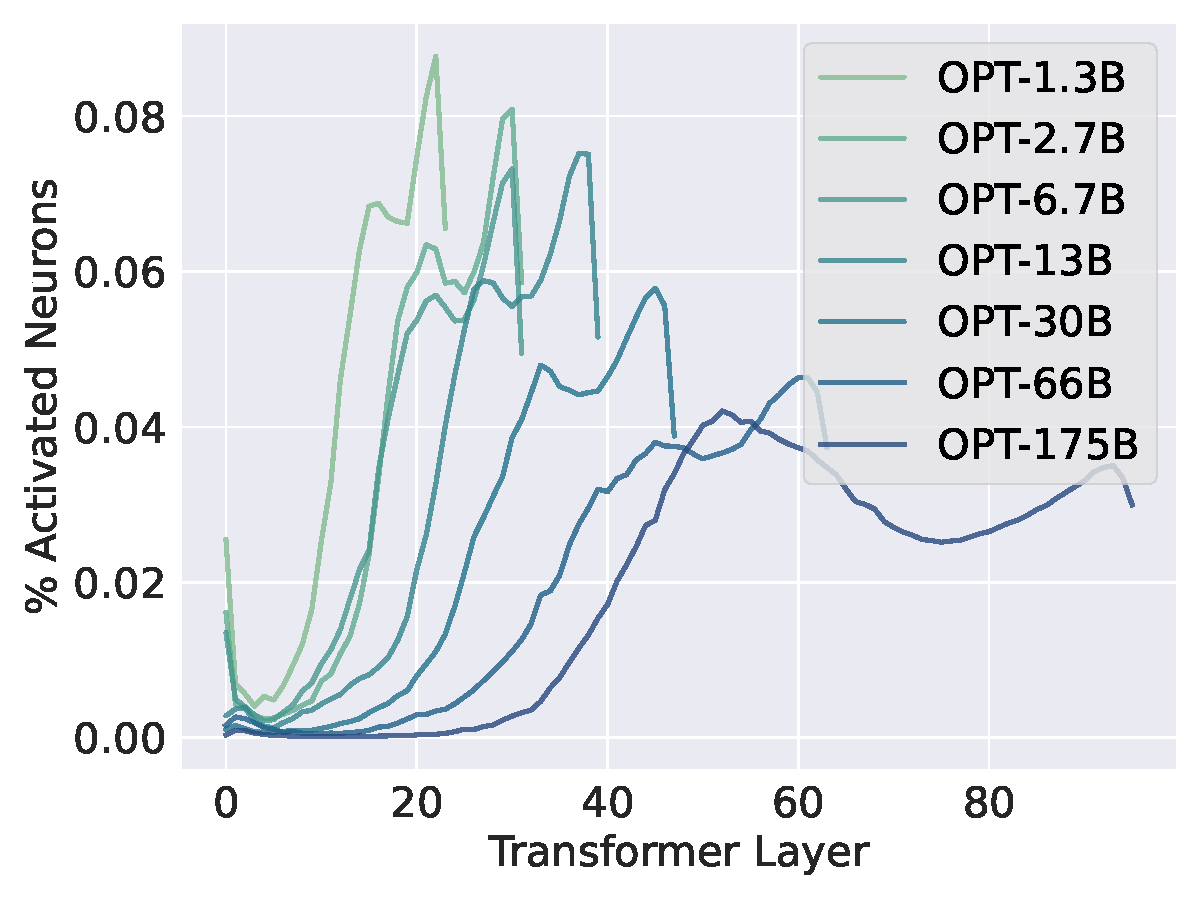
\includegraphics[width=0.4\textwidth]{figure/observation/mlp_sparsity.pdf}
%     \label{fig:sparsity-mlp}
%   }
%     \subfigure[Dynamic Sparsity]{
%     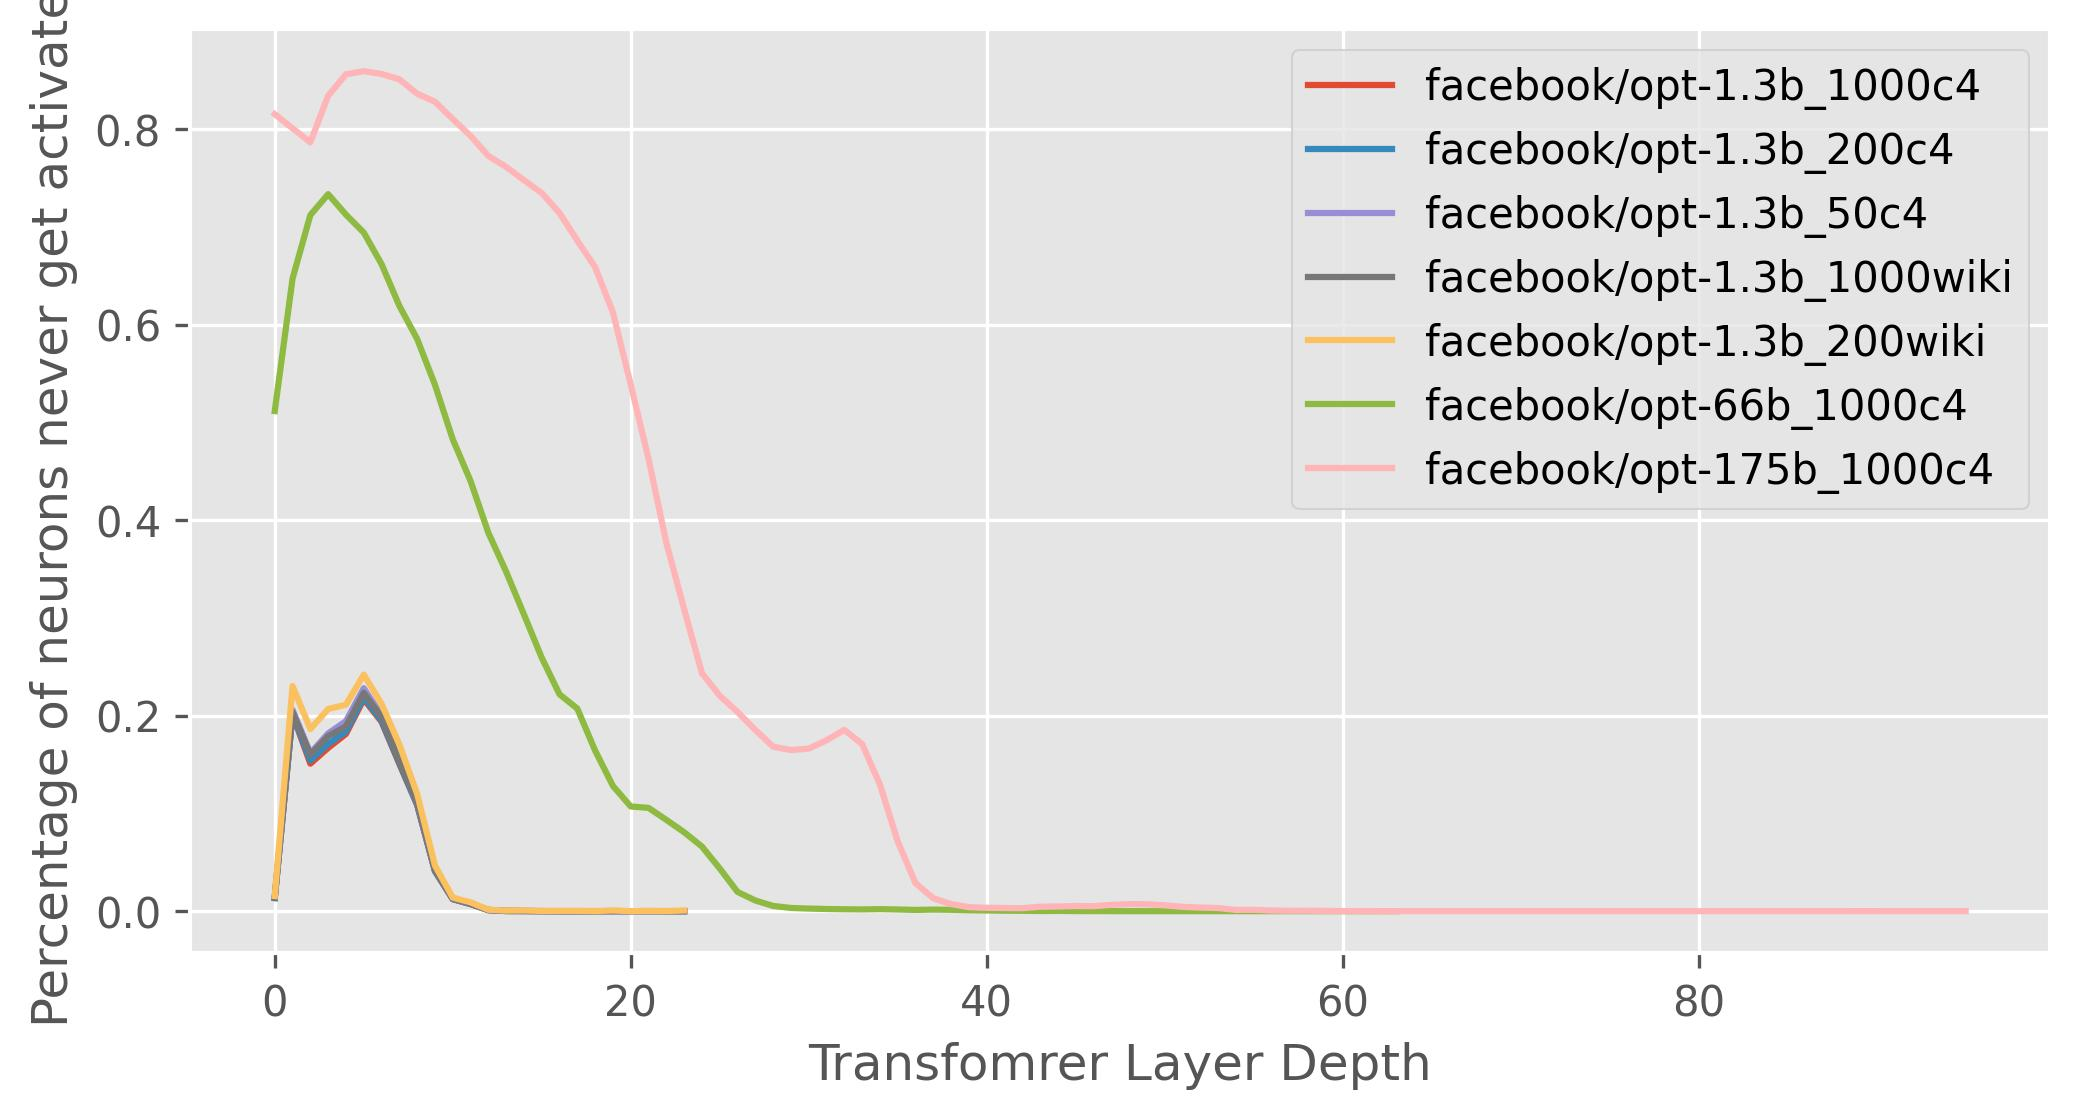
\includegraphics[width=0.4\textwidth]{figure/observation/neuron_activation.jpeg}
%     \label{fig:dynamic-sparsity} 
%   }
%   \caption{ \textbf{High sparsity in the MLP block} The percentage of activated neurons after the activation function in the MLP block is less than 10\% across models and across layers. The percentage is lower for larger models.  }
%   \label{observation:sparsity} 
% \end{figure}

% The research community often regards high sparsity as a promising opportunity for efficiency~\cite{https://doi.org/10.48550/arxiv.2210.06313}. 
% However, due to the nature of dynamic sparsity, it requires an adaptive selection of neurons to the input tokens for inference.
% Approximate nearest neighbor search (NNS) is a widely established solution for exploiting dynamic sparsity for inference efficiency. 
% The computation of the Expand MLP is given by the following equation:
% \begin{equation*}
%     \sigma(W^Tx)
% \end{equation*}
% where $x \in R^d$ is the input to the layer and $W \in R^{d \times 4d}$ are the weights of the Expand-MLP, with each row $w_i \in \R^{d}, i \in [4d]$ corresponding to the weight of the $i$-th neuron. Instead of computing the matrix multiplication at Expand MLP, given the high sparsity, approximate-NNS methods can be used to find  $k$ near neurons $\{w_i \}_1^k$ measured by the inner product. Approximate-NNS methods enjoy sub-linear complexity and reduce the matrix multiplication from the dimension $4d$ to $k$.  However, despite the theoretical saving in FLOPs, it is challenging to achieve wall-clock inference time reduction in large language models. On the one hand, due to the high dimensionality of $x$, e.g.~$d = 12288$ in OPT-175b, approximate-NNS methods incur long query time for high recall.  On the other hand, large language model inferences are performed on modern accelerators such as NVIDIA A100, which are blazing fast in computing matrix multiplication. In many cases, the query overhead may even be longer than computing the matrix multiplication in the original dimension.


% We argue that waiting for the input to the Expand-MLP layer as the query is unnecessary. Our argument is based on the following observation:
% \begin{center}
%     Activation evolves \emph{extremely slowly} in LLMs. 
% \end{center} 
% We record the hidden states throughout the model and compute the cosine distance between the hidden states. Taking OPT-175b as an example, we found that (1) the cosine similarity between the input of the MHA block and the MLP block within the same transformer layer is over 99\%. (2) the cosine similarity between the input of any two consecutive transformer layers is over 98\%. 
% \emma{TODO: cannot follow here.}
% We estimate that eliminating the query overhead could result in 2.5 $\times$ reduction in end-to-end inference time. In contrast, we show in Section~\ref{} that the naive adoption of approximate-NNS methods increases the wall clock time.

% We demonstrate that the slowly evolving activations presented in large language models provide opportunities for reducing wall-clock inference time. By exploiting the activations of the previous block or layer, we can parallelize the query process with model computation to avoid the query overhead from its sequential nature. However, several challenges remain: (1) Characterizing the slowly evolving activations, (2) Identifying the appropriate approximate-NNS method to exploit hardware characteristics, and (3) Addressing unstructured sparsity in implementation for systemic improvement.

% In this paper, we propose Deja Vu, a framework to achieve efficient inference with large language models by reducing both the width and depth.  We show one major observation, slowly changing activation, and two key algorithm
% based on it in Deja Vu. Specifically,

% \begin{itemize}
% \item In Section~\ref{}, we measure the differences between activations during the inference process. We find that the activations are slowly evolving, and formally define this small evolving phenomena in Assumption ~\ref{}, which is the foundation to build Deja Vu.


% \item In Section~\ref{}, we present an algorithm for paralleling blocks inside LLMs. Under slow evloving activation assumption, we show that (some theory result?)


% \item In Section~\ref{}, we propose a method for adaptively selecting a subset of neurons in MLP blocks. Our method uses the activations from the previous layer as the query to avoid overhead.  

% \item In Section, we demonstrate the efficiency of Deja Vu on LLMs. When applied to OPT-175b,  we show $\times$ speed up in time without losses on accuracy. When applied to Bloom, we show that 
% \end{itemize}


% \begin{figure*}[]
%   \centering
%  \subfigure[]{
%     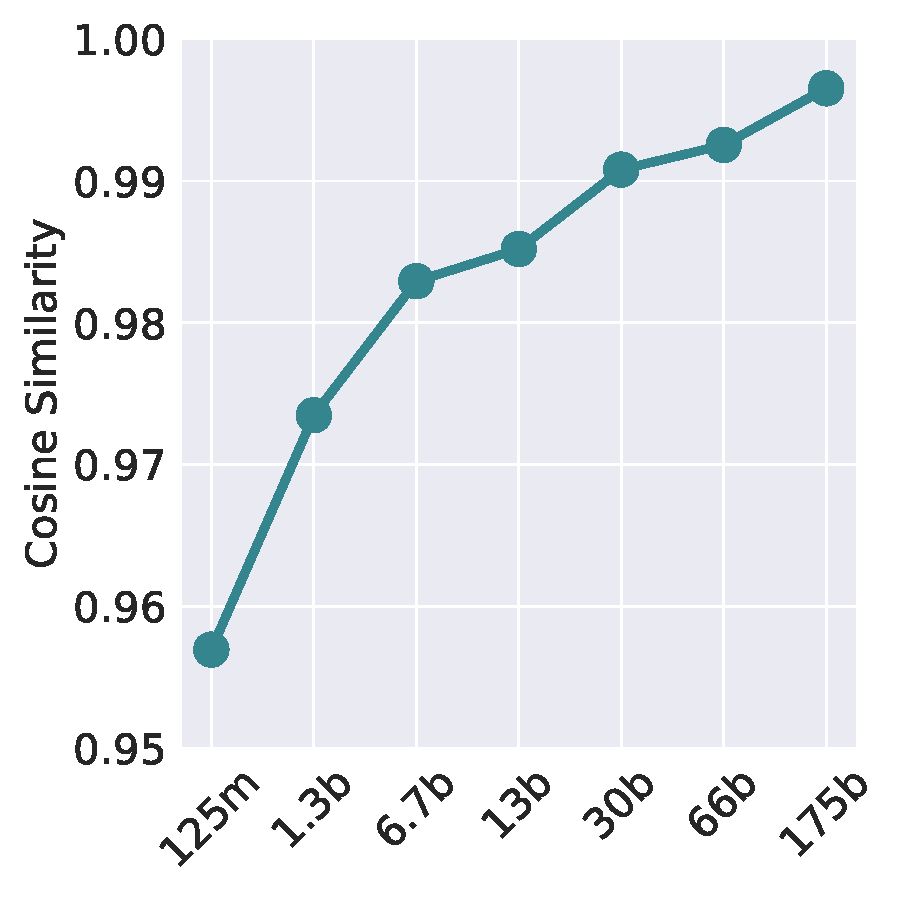
\includegraphics[width=0.23\textwidth]{figure/observation/cos_across_model.pdf}
%     \label{obs:slowlyevoloving-all}
%     }
%   \subfigure[OPT-1.3B]{
%     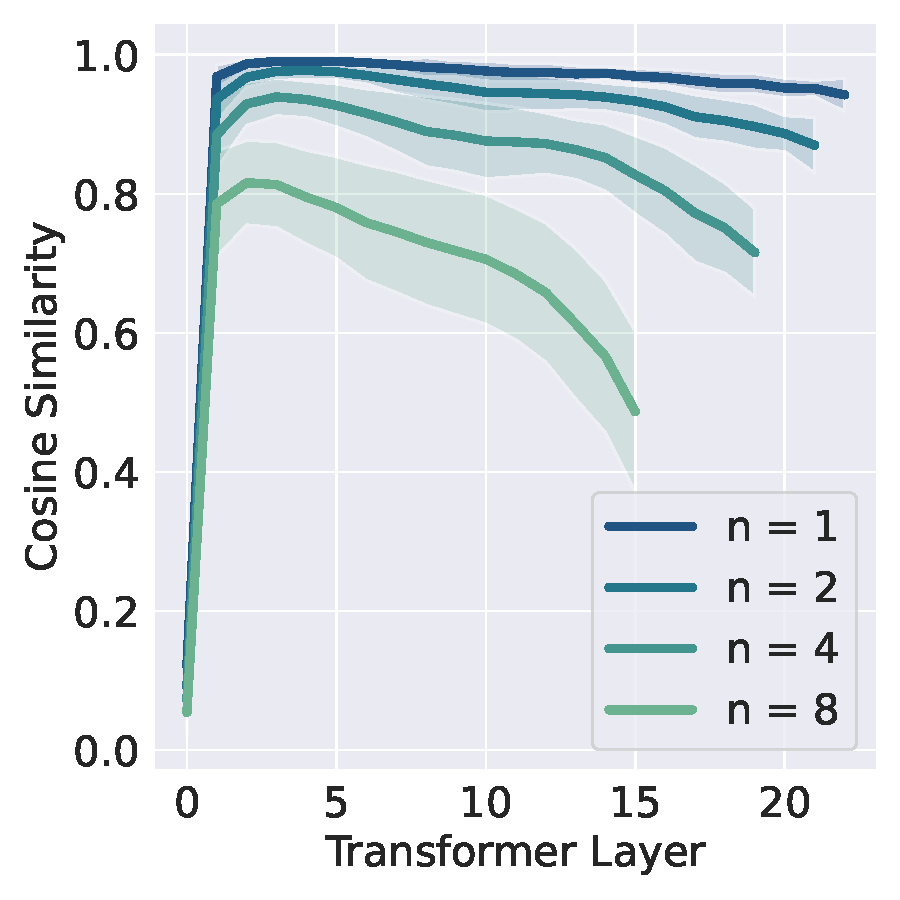
\includegraphics[width=0.23\textwidth]{figure/observation/1.3b_between_layer_cos.pdf}
%     \label{obs:slowlyevoloving-125m}
%   }
%     \subfigure[OPT-30B]{
%     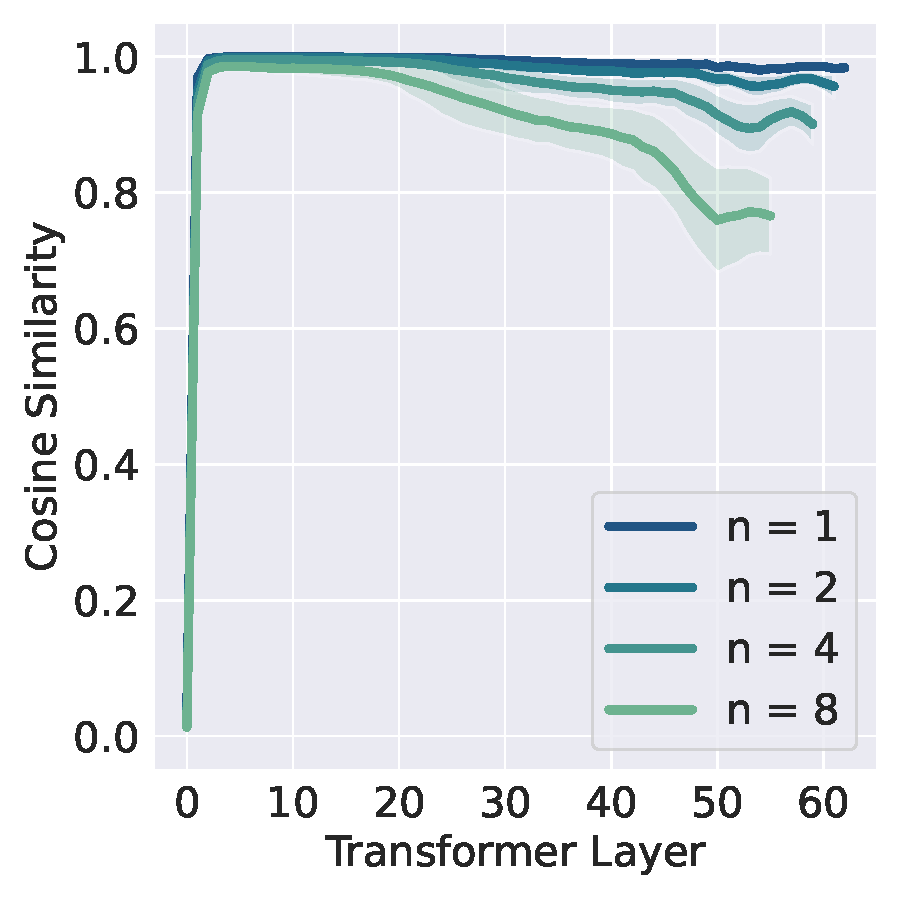
\includegraphics[width=0.23\textwidth]{figure/observation/66b_between_layer_cos.pdf}
%     \label{obs:slowlyevoloving-30b}
%   }
%   \subfigure[OPT-175B]{
%     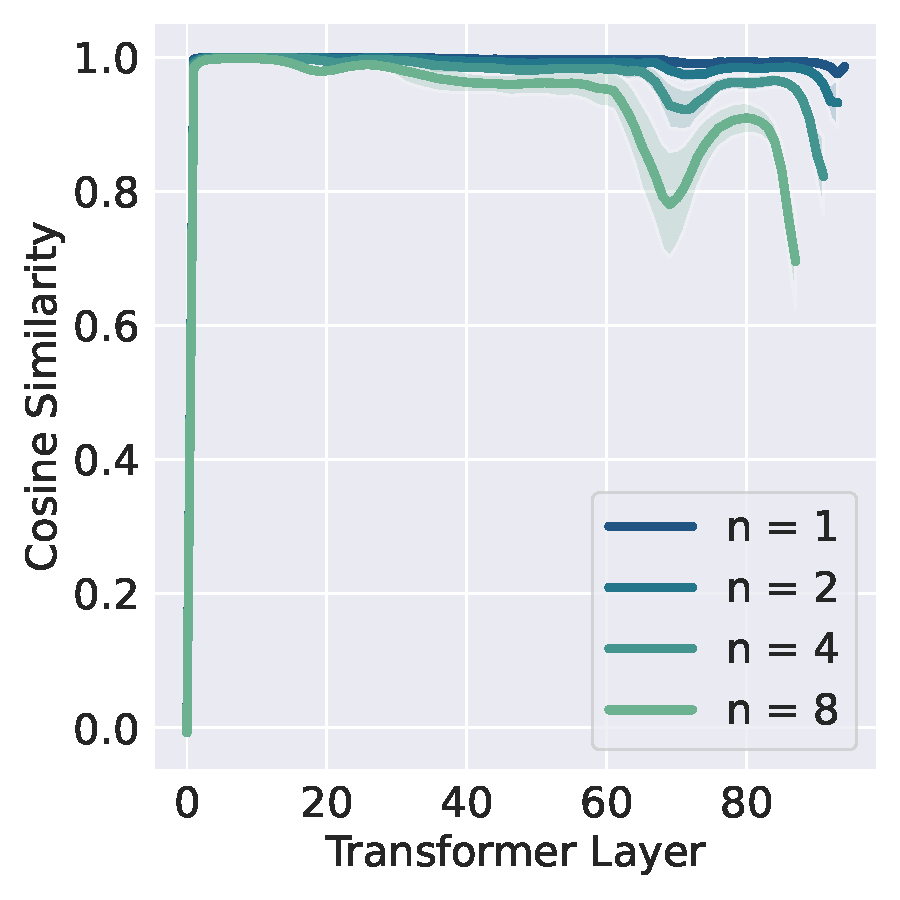
\includegraphics[width=0.23\textwidth]{figure/observation/175b_between_layer_cos.pdf}
%     \label{obs:slowlyevoloving-175b}
%   }
%   \caption{ \textbf{Slowly Evolving Representation: } We look at the cosine similarity between representations at transformer layer $i$ and transformer layer $i + n$ for the same input.  Figure (a) shows the median cosine similarity between representations at two consecutive layers ($n = 1$) across all layers for different OPT models. All models show a similarity greater than 95\%. Also, similarity increases as the model grow larger. Figure (b), (c), and (d) shows the cosine similarity with various choices of $n$ at every layer. The similarity is near zero at the first layer. Starting at the second layer, cosine similarity remains high and drops a little at later layers. The similarity is lower when $n$ is larger.  }
%   \label{obs:slowlyevoloving} 
% \end{figure*}
% \vspace{-6mm}
% \begin{figure*}[]
%   \centering

%   \subfigure[OPT-1.3B]{%
%     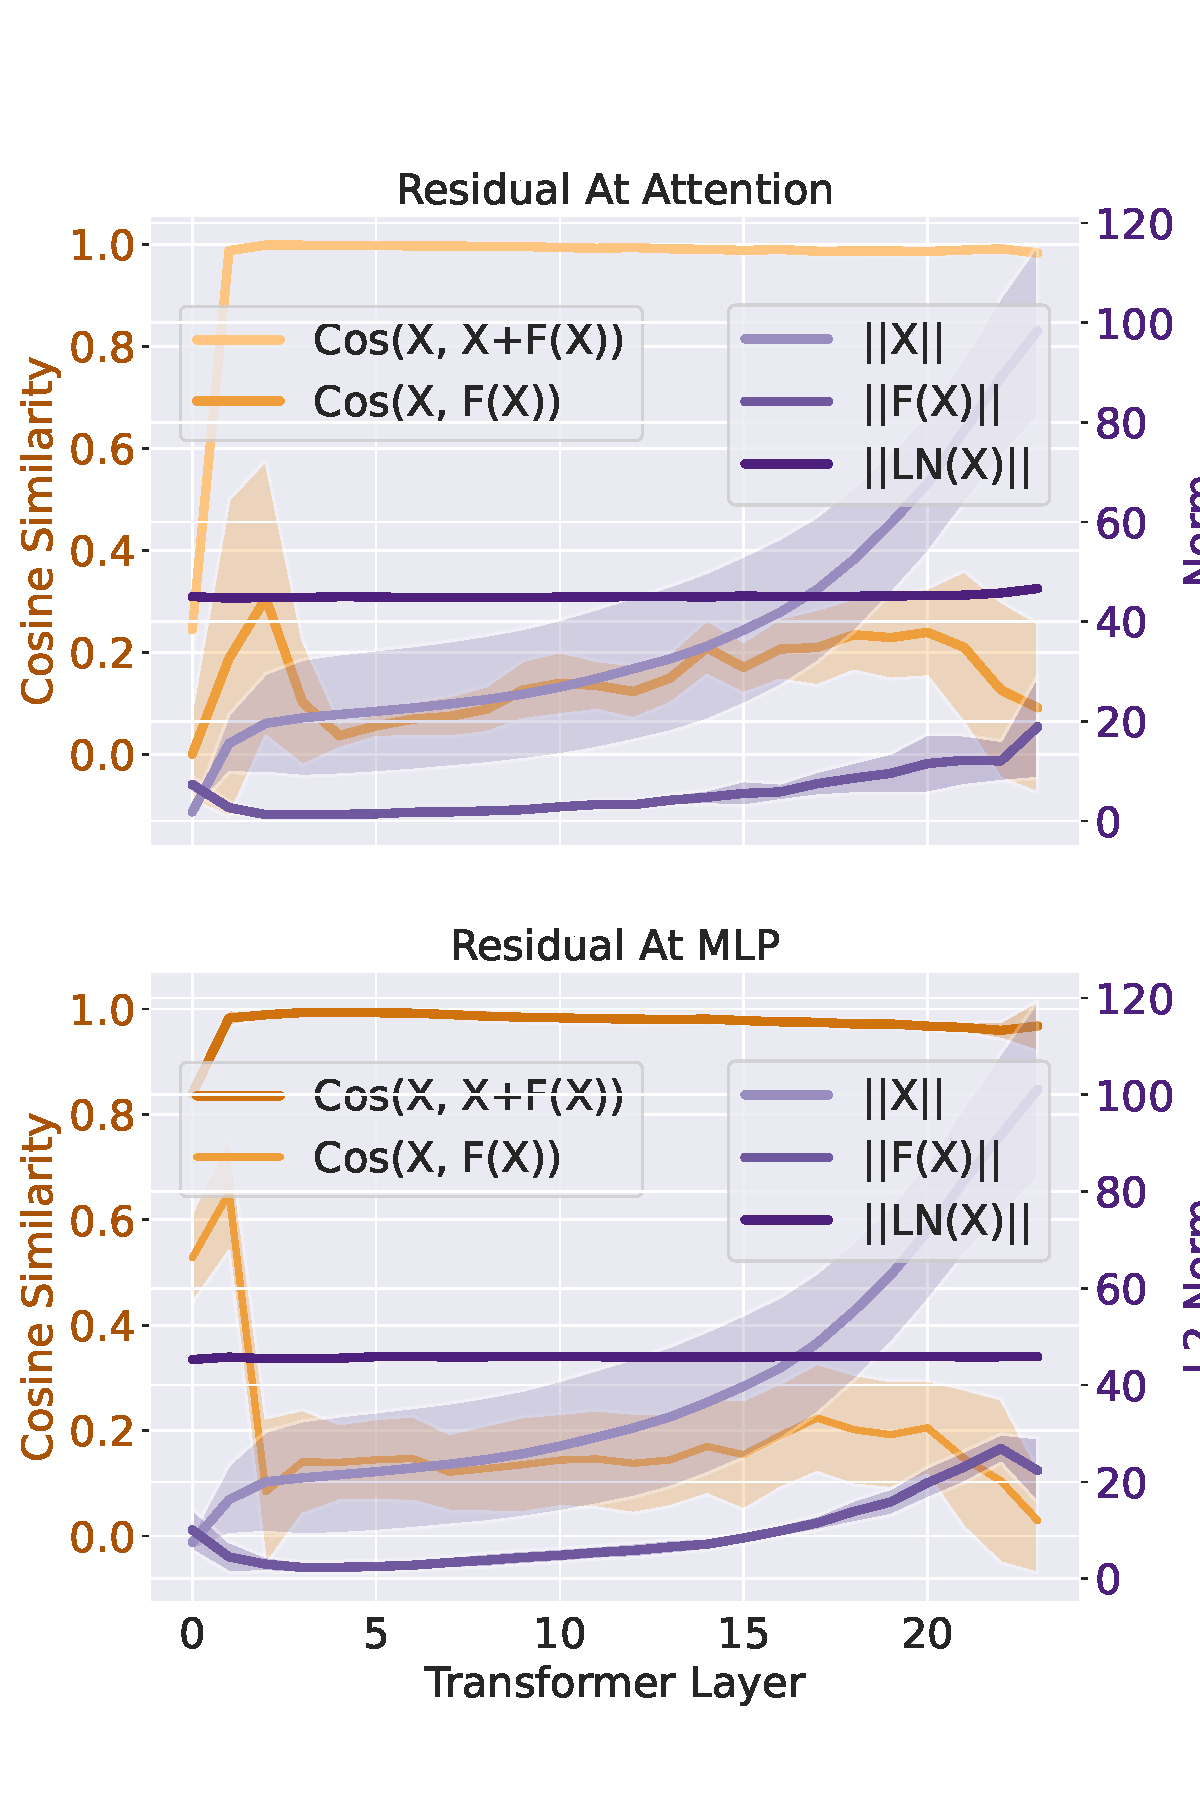
\includegraphics[width=0.33\textwidth]{figure/observation/1.3b_residual_before_after.pdf}%
%   }%
% %   \hfill
%   \subfigure[OPT-30B]{%
%     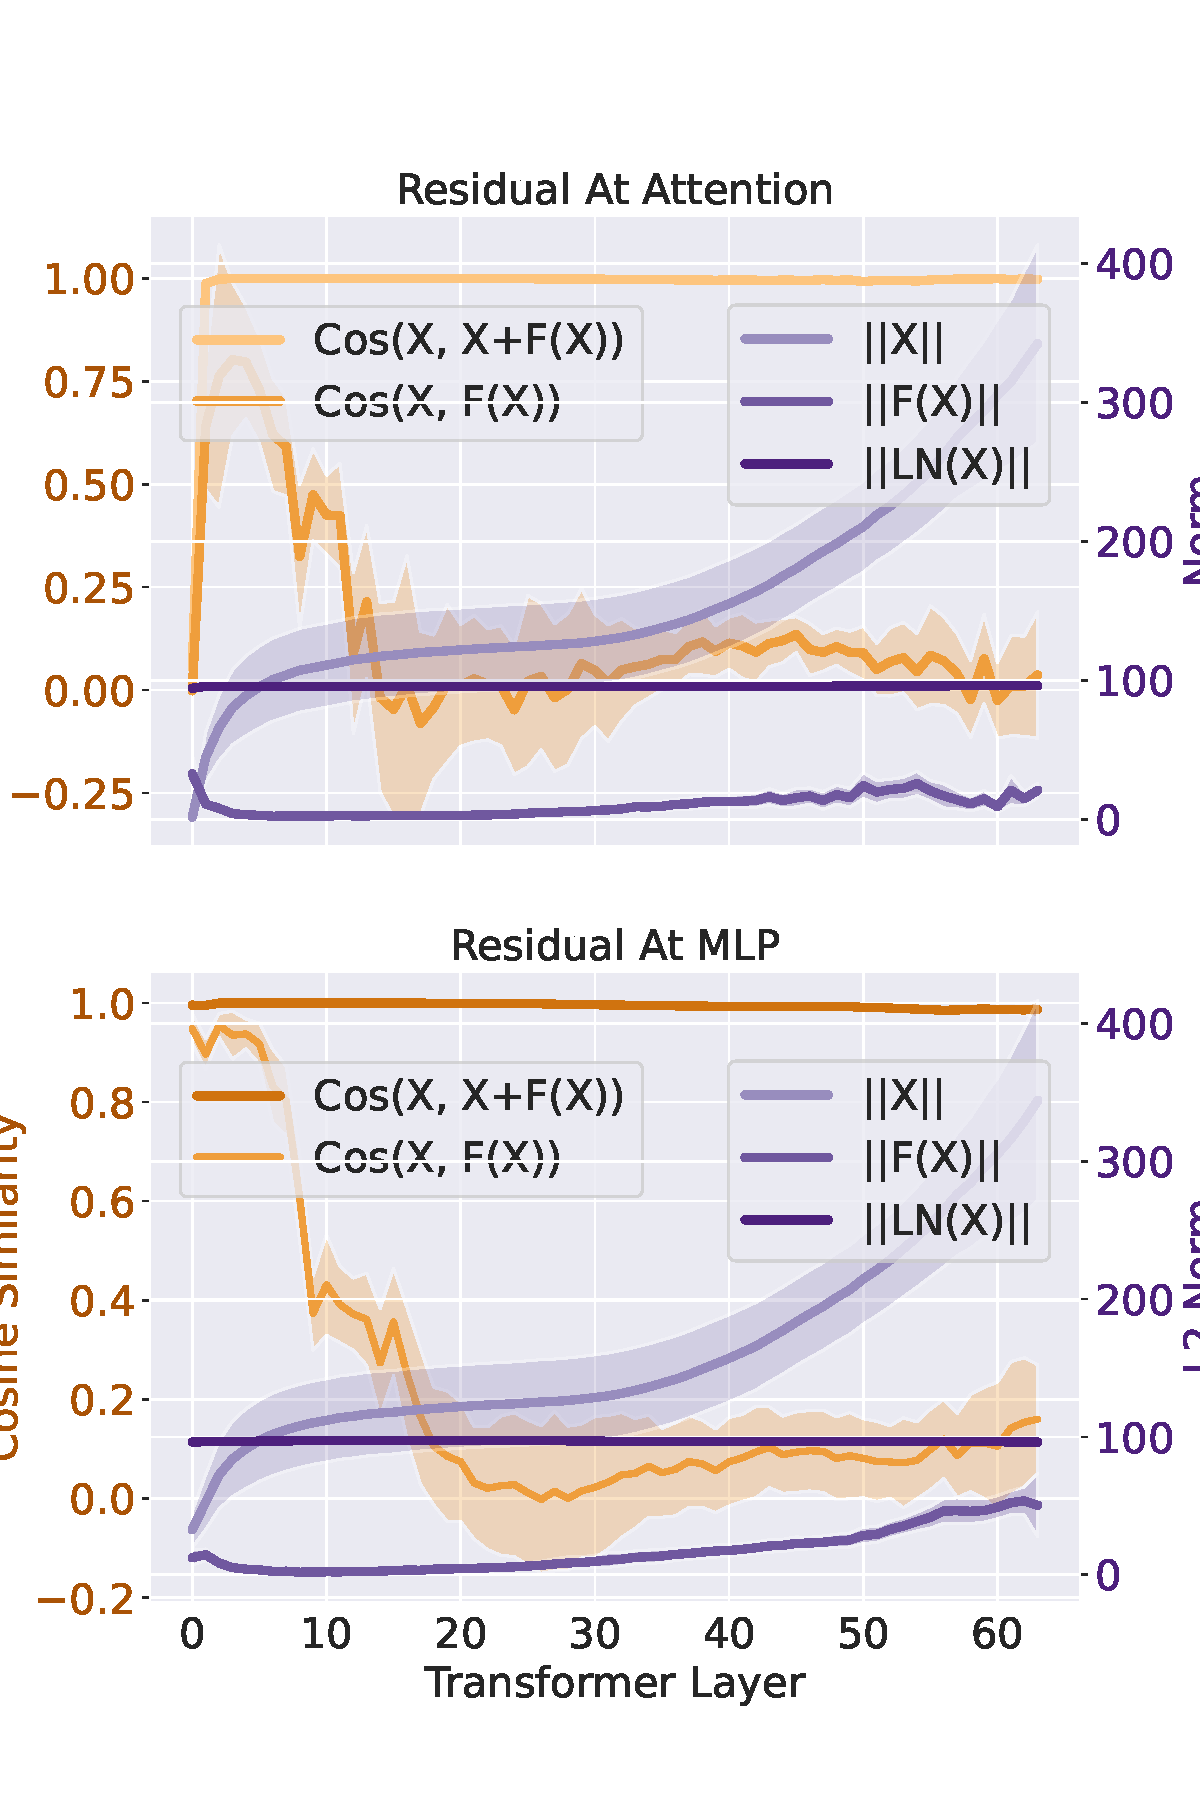
\includegraphics[width=0.33\textwidth]{figure/observation/66b_residual_before_after.pdf}%
%   }%
%     \subfigure[OPT-175B]{%
%     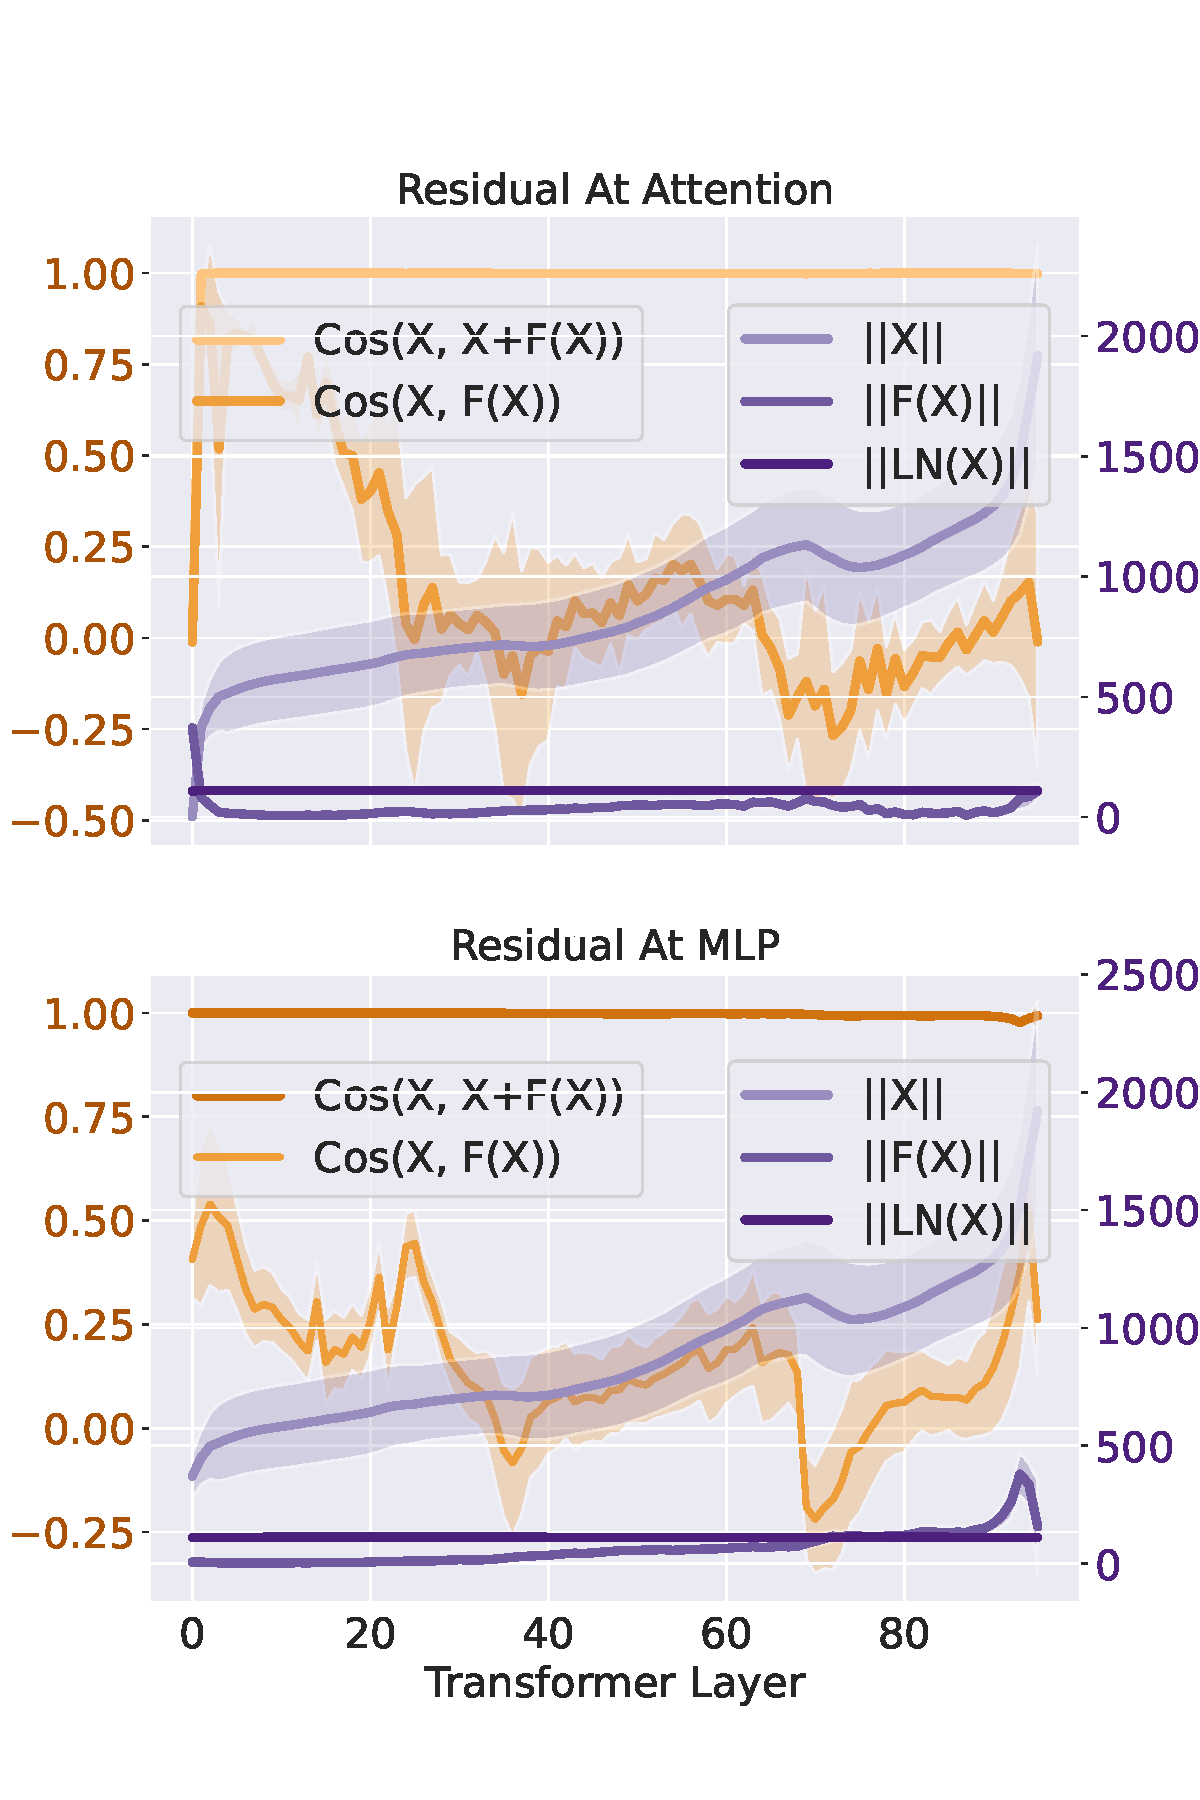
\includegraphics[width=0.33\textwidth]{figure/observation/175b_residual_before_after.pdf}%
%   }%
%   \caption{ \textbf{Residual connection maintains the angle.} There are two residual connections $X' = X + F(X)$ inside each transformer layer, one around the attention block and one around the MLP block. In this figure, we plot the cosine similarity between $X$ and $F(X)$, and the cosine similarity between $X$ and $X'$ in orange color. The similarity between $X'$ and $X$ is extremely high at all layers( except the first layer), while the similarity between $X$ and $F(X)$ is low, almost orthogonal in the majority of layers. To explain this, we plot the $L2$ norm of $X$ and $F(X)$. Except on the first layer, $\|X\|$ is significantly higher than $\|F(X)$. $\|F(X)\|$ is higher at the first layer, which corresponds to the low cosine similarity at the first layer. }
%   \label{observation:residual} 
% \end{figure*}

%%% Local Variables:
%%% mode: latex
%%% TeX-master: "main"
%%% End:
